\documentclass[12pt,a4paper]{report}

%% ─── Packages ────────────────────────────────────────────────────────────────
\usepackage[margin=2.5cm]{geometry}
\usepackage[T1]{fontenc}
\usepackage[utf8]{inputenc}
\setlength{\headheight}{14pt}
\usepackage{graphicx}
\usepackage{hyperref}
\usepackage{titlesec}
\usepackage{enumitem}
\usepackage{booktabs}
\usepackage{longtable}
\usepackage{array}
\usepackage{multirow}
\usepackage{xcolor}
\usepackage{fancyhdr}
\usepackage{setspace}
\usepackage{parskip}
\usepackage{caption}
\usepackage{float}
\usepackage{microtype}
\usepackage{tikz}
\usetikzlibrary{shapes.geometric, arrows.meta, positioning, backgrounds}

%% ─── Colours ─────────────────────────────────────────────────────────────────
\definecolor{primary}{RGB}{37,99,235}
\definecolor{light}{RGB}{239,246,255}
\definecolor{dark}{RGB}{30,41,59}
\definecolor{accent}{RGB}{16,185,129}

%% ─── Hyperref ────────────────────────────────────────────────────────────────
\hypersetup{
  colorlinks=true, linkcolor=primary, urlcolor=primary,
  pdftitle={GoPlay Sports Platform -- Final Report},
  pdfauthor={Team GoPlay}
}

%% ─── Header / Footer ─────────────────────────────────────────────────────────
\pagestyle{fancy}\fancyhf{}
\fancyhead[L]{\small GoPlay Sports Platform}
\fancyhead[R]{\small Final Project Report}
\fancyfoot[C]{\thepage}
\renewcommand{\headrulewidth}{0.4pt}

%% ─── Chapter / Section titles ────────────────────────────────────────────────
\titleformat{\chapter}[display]
  {\normalfont\Large\bfseries\color{primary}}{\chaptertitlename\ \thechapter}
  {10pt}{\huge}
\titlespacing*{\chapter}{0pt}{20pt}{20pt}
\titleformat{\section}{\large\bfseries\color{dark}}{}{0em}{\thesection\quad}
\titleformat{\subsection}{\normalsize\bfseries}{}{0em}{\thesubsection\quad}

\onehalfspacing

%% =============================================================================
\begin{document}

%% ─── Title Page ──────────────────────────────────────────────────────────────
\begin{titlepage}
\centering\vspace*{1.5cm}
{\Huge\bfseries\color{primary} GoPlay Sports Platform}\\[0.8cm]
{\LARGE Final Project Report}\\[1.5cm]
\rule{\textwidth}{1.5pt}\\[0.5cm]
{\large\bfseries Submitted in partial fulfilment of the requirements\\
for the Software Engineering Module}\\[0.5cm]
\rule{\textwidth}{1.5pt}\\[2cm]

\begin{tabular}{lll}
\toprule
\textbf{Name} & \textbf{Module(s)} & \textbf{Contribution}\\
\midrule
Malika Nishnatha   & User Module \& Ground Owner Module & 30\%\\
Winuka Mahagamage  & Coach Module                       & 25\%\\
Ravindu            & Admin Module \& News CRUD           & 25\%\\
Piyumi             & Shop Owner Module                  & 20\%\\
\bottomrule
\end{tabular}

\vfill
{\large Academic Year 2025/2026}\\[0.3cm]
{\large April 2026}
\end{titlepage}

\tableofcontents\newpage

%% =============================================================================
\chapter{Introduction}
%% =============================================================================

\section{Domain Description}

Sports participation is a rapidly growing activity in Sri Lanka, spanning recreational players, competitive athletes, and professional coaches across disciplines such as cricket, football, basketball, tennis, badminton, swimming, and volleyball. Despite this growth, accessing sports infrastructure remains fragmented: booking a ground requires a phone call, finding a qualified coach depends on word of mouth, purchasing equipment means visiting scattered physical stores, and there is no single trusted hub for Sri Lankan sports news.

\textbf{GoPlay Sports Platform} is a web-based multi-role sports marketplace designed to bridge these gaps. It unifies four provider types — ground owners, professional coaches, sports equipment shop owners, and a platform administrator — with end users (players) under a single digital ecosystem. Users can discover and book sports facilities, hire professional coaches, purchase sporting goods, and follow local sports news, all from one platform.

\section{Current System and Limitations}

Prior to GoPlay, the Sri Lankan sports community relied on informal, manual processes that suffered from the following limitations:

\begin{itemize}[leftmargin=1.5cm]
  \item \textbf{Manual Ground Booking:} Players contacted facility owners by telephone or walked in to check availability and reserve time slots. No real-time availability was visible, and double-bookings were common.
  \item \textbf{No Centralised Coach Directory:} There was no reliable way to discover, vet, or book professional coaches. Players relied entirely on personal networks.
  \item \textbf{Scattered Equipment Purchase:} Purchasing sports equipment required visiting multiple physical stores with no online catalog, price comparison, or delivery option.
  \item \textbf{No Digital Earnings Tracking:} Ground owners and coaches had no automated tools to track their income, outstanding bookings, or revenue trends.
  \item \textbf{No Maintenance or Inspection Records:} Ground owners managed facility upkeep informally, with no digital records of maintenance tasks, schedules, or safety inspections.
  \item \textbf{No Provider Onboarding Workflow:} There was no standardised process for verifying and onboarding new ground owners, coaches, or shop owners.
  \item \textbf{No Centralised Sports News:} Sports news was scattered across social media and general news sites with no local sports-specific hub.
\end{itemize}

\section{Goals and Objectives}

The primary goal of GoPlay is to digitise and streamline the Sri Lankan sports ecosystem for all stakeholders. The specific objectives are:

\begin{enumerate}[leftmargin=1.5cm]
  \item Provide a real-time online ground booking system with availability checking and slot-based reservations.
  \item Establish a coach discovery, profile, and booking platform.
  \item Deliver a multi-vendor sports equipment e-commerce system with cart, checkout, and order tracking.
  \item Give ground owners a full management portal: grounds, bookings, availability, maintenance, inspections, earnings, and reviews.
  \item Give coaches a management portal: profile, credentials, session scheduling, client tracking, and earnings.
  \item Give shop owners a management portal: product catalog, inventory, orders, and reviews.
  \item Provide administrators with a centralised panel to manage users, approve providers, oversee platform earnings, and publish sports news.
  \item Integrate the PayHere payment gateway for secure online transactions.
  \item Implement a review and rating system for facilities, coaches, and products.
  \item Implement a notification system for all stakeholders (bookings, orders, reviews, approvals).
  \item Implement detailed analytics and activity logging for the admin.
\end{enumerate}

\section{Process Re-Engineering}

GoPlay re-engineers the following real-world processes:

\begin{center}
\begin{tabular}{p{5.5cm} p{8.5cm}}
\toprule
\textbf{Old Process} & \textbf{Re-Engineered Process on GoPlay}\\
\midrule
Phone/walk-in ground booking & Online booking with real-time slot availability and instant confirmation\\
Word-of-mouth coach discovery & Searchable coach profiles with credentials, ratings, and direct session booking\\
Cash/in-person equipment purchase & Online shop with cart, checkout, and PayHere/COD payment\\
Manual earnings record-keeping & Automated earnings dashboards with period filters and export\\
Ad-hoc maintenance scheduling & Digital maintenance task management with progress tracking and inspection records\\
Informal provider onboarding & Structured online application with document upload and admin approval workflow\\
Scattered sports news & Admin-curated news portal with categories, featured articles, search, and view analytics\\
No review mechanism & Structured review and rating system for grounds, coaches, and products with reply/report features\\
\bottomrule
\end{tabular}
\end{center}

\section{Assumptions}

\begin{itemize}[leftmargin=1.5cm]
  \item All users have access to a modern web browser and a stable internet connection.
  \item Ground owners have legitimate ownership or management rights over the facilities they register.
  \item Coaches possess the qualifications and certifications they declare on their profiles.
  \item The PayHere payment gateway is configured with valid merchant credentials in the deployment environment.
  \item The platform is deployed on a server running PHP 8.x and MySQL 8.x.
  \item All monetary amounts are in Sri Lankan Rupees (LKR / Rs.).
  \item Provider applications are reviewed and acted upon by a human administrator.
\end{itemize}

%% =============================================================================
\chapter{Feasibility Study}
%% =============================================================================

\section{Technical Feasibility}

GoPlay is built on a proven, widely supported open-source stack:

\begin{itemize}[leftmargin=1.5cm]
  \item \textbf{Backend:} PHP 8.x with a custom MVC framework (no third-party framework dependency), giving full control over routing, request handling, and session management.
  \item \textbf{Database:} MySQL 8.x with PDO for all queries, supporting transactions needed for booking and payment atomicity.
  \item \textbf{Security:} Passwords hashed with \texttt{PASSWORD\_ARGON2ID}. Login history, user activity, and admin action logs are recorded in dedicated tables.
  \item \textbf{Frontend:} HTML5, CSS3, and vanilla JavaScript. No heavy frontend framework is required, keeping the application lightweight and fast.
  \item \textbf{Email:} PHPMailer for transactional emails (booking confirmations, provider approval/rejection notifications).
  \item \textbf{Payment:} PayHere, a Sri Lanka-based payment gateway with a documented PHP integration and webhook support.
  \item \textbf{File Uploads:} Provider application documents, product images, profile avatars, and shop logos stored on the server filesystem.
\end{itemize}

All team members have the required PHP and MySQL skills. The chosen stack is deployable on affordable shared or VPS hosting available in Sri Lanka.

\section{Economic Feasibility}

\begin{itemize}[leftmargin=1.5cm]
  \item \textbf{Development Cost:} Zero monetary cost; the project uses free and open-source tools (PHP, MySQL, VS Code, draw.io).
  \item \textbf{Hosting Cost:} A VPS or shared hosting plan (approximately Rs.\ 2,000--5,000 per month) is sufficient.
  \item \textbf{Revenue Model (future):} The platform already tracks service fees via a \texttt{platform\_earnings} table and includes a withdrawal request system, enabling a commission-based revenue model in production.
\end{itemize}

\section{Operational Feasibility}

\begin{itemize}[leftmargin=1.5cm]
  \item Each role has a dedicated dashboard with a consistent, intuitive sidebar navigation, minimising the learning curve.
  \item The admin panel provides complete oversight of all platform activity without requiring technical knowledge.
  \item Ground owners can manage all aspects of their facilities independently, reducing administrative overhead.
  \item Coaches self-manage their profiles, availability, and sessions, scaling with no manual coordination.
\end{itemize}

\section{Schedule Feasibility}

The project was divided into four independent modules (User/Ground Owner, Coach, Admin/News, Shop Owner) assigned to individual team members, enabling fully parallel development. The MVC architecture ensured that model, view, and controller layers of each module could be developed independently without blocking dependencies on other modules.

%% =============================================================================
\chapter{Requirements}
%% =============================================================================

\section{Stakeholders / Actors}

\begin{center}
\begin{tabular}{p{3.2cm} p{10.8cm}}
\toprule
\textbf{Actor} & \textbf{Description}\\
\midrule
\textbf{Guest / Visitor}  & Any unauthenticated user. Can browse the homepage, view facilities, coach listings, news, and the public shop. Cannot book or purchase.\\
\textbf{Registered User}  & Authenticated platform member. Can book grounds, hire coaches, purchase equipment, submit reviews, manage their profile, and track notifications.\\
\textbf{Ground Owner}     & Approved facility manager. Manages facility listings, bookings, availability, maintenance, inspections, earnings, reviews, and coach enrollments.\\
\textbf{Coach}            & Approved sports professional. Manages their profile, certificates, availability, sessions, clients, earnings, and facility connections.\\
\textbf{Shop Owner}       & Approved sports equipment retailer. Manages product catalog, inventory, orders, reviews, and shop profile.\\
\textbf{Administrator}    & Platform superuser. Approves provider applications, manages users, oversees payments and platform earnings, and publishes sports news.\\
\bottomrule
\end{tabular}
\end{center}

\section{Functional Requirements}

\subsection{User Module (Malika Nishnatha)}

\begin{enumerate}[leftmargin=1.5cm]
  \item The system shall allow users to register with their first name, last name, email, and password.
  \item The system shall authenticate users via email and password with secure session management.
  \item The system shall display a personalised dashboard showing ground booking count, coach session count, order count, and recent activity.
  \item The system shall allow users to browse sports facilities by sport type and location with real-time availability checking.
  \item The system shall allow users to book a sports facility by selecting a date and available time slot.
  \item The system shall allow users to browse and book coach sessions via a public coach profile page.
  \item The system shall allow users to view and manage their ground bookings and coach sessions (reschedule, cancel).
  \item The system shall provide a persistent shopping cart (for both guest and authenticated users with merge on login).
  \item The system shall provide a multi-step checkout: contact details $\to$ payment method $\to$ payment processing $\to$ order confirmation.
  \item The system shall support three payment methods: Cash on Delivery, Card, and PayHere gateway.
  \item The system shall allow users to view order history with per-order item details.
  \item The system shall allow users to update their profile, change their password, and upload a profile picture.
  \item The system shall deliver in-app notifications for booking confirmations, order updates, and coach session changes.
  \item The system shall allow users to submit star ratings and text reviews for sports facilities.
\end{enumerate}

\subsection{Ground Owner Module (Malika Nishnatha)}

\begin{enumerate}[leftmargin=1.5cm]
  \item The system shall allow users to apply as ground owners with supporting documents.
  \item The system shall allow approved ground owners to create, update, and delete sports facility listings.
  \item The system shall allow ground owners to configure weekly availability schedules and block specific dates.
  \item The system shall allow ground owners to view, filter, and manage all facility bookings.
  \item The system shall display ground owner earnings with breakdown by period and per-facility.
  \item The system shall allow ground owners to create, track, and update maintenance tasks with progress notes.
  \item The system shall allow ground owners to schedule and record facility safety inspections with health scores.
  \item The system shall allow ground owners to reply to and report user reviews on their facilities.
  \item The system shall allow ground owners to view coach enrollment requests (pending/approved/rejected) and approve or reject them, triggering a notification to the coach.
  \item The system shall display an overall schedule view of all upcoming bookings across all facilities.
  \item The system shall allow ground owners to manage their profile and account settings.
\end{enumerate}

\subsection{Coach Module (Winuka Mahagamage)}

\begin{enumerate}[leftmargin=1.5cm]
  \item The system shall allow coaches to maintain a professional profile (bio, specialisations, experience, hourly rate, avatar).
  \item The system shall allow coaches to add, edit, and delete professional certificates and achievements.
  \item The system shall allow coaches to set a weekly availability schedule with per-day time ranges.
  \item The system shall display a monthly calendar view with booked-date badges and an upcoming sessions list.
  \item The system shall allow coaches to view, confirm, mark as complete, and cancel their sessions.
  \item The system shall display a client management dashboard with a client list, per-client booking history, and CSV export.
  \item The system shall display a coach earnings dashboard showing per-session income, totals, and trends in LKR.
  \item The system shall allow coaches to respond to reviews left by users.
  \item The system shall allow coaches to link their profile to sports facilities (pending/approved/rejected status), set a primary facility, and unlink facilities.
  \item The system shall provide a public coach profile page for users to view credentials, reviews, and available time slots.
  \item The system shall support a bundled booking (coach session + linked facility slot) as a single atomic transaction.
\end{enumerate}

\subsection{Admin Module (Ravindu)}

\begin{enumerate}[leftmargin=1.5cm]
  \item The system shall provide an admin dashboard with platform-wide KPI statistics.
  \item The system shall allow administrators to list, search, filter, and view all provider applications (ground owners, coaches, shop owners) and approve or reject them with automated email notification.
  \item The system shall allow administrators to manage registered user accounts (view details, update roles, reset passwords, delete accounts).
  \item The system shall allow administrators to view platform payment records and manage earnings.
  \item The system shall allow administrators to process and manage provider withdrawal requests.
  \item The system shall provide a full analytics dashboard (user growth, revenue trends, booking activity, product performance, activity logs) with export capability.
  \item The system shall allow administrators to manage system settings including service fee configuration, email testing, and database backup.
  \item The system shall allow administrators to create, edit, publish/unpublish, and delete sports news articles with category and featured-article support.
  \item The system shall allow administrators to track trending news and view article engagement analytics.
\end{enumerate}

\subsection{Shop Owner Module (Piyumi)}

\begin{enumerate}[leftmargin=1.5cm]
  \item The system shall display a shop owner dashboard with product stats, order stats, revenue, low-stock alerts, recent orders, top-selling products, and recent reviews.
  \item The system shall allow shop owners to add, edit, and delete product listings with images, descriptions, pricing, and category assignment.
  \item The system shall allow shop owners to manage product inventory with minimum stock thresholds and low-stock alerts.
  \item The system shall allow shop owners to view and update customer order statuses (pending $\to$ processing $\to$ shipped $\to$ delivered).
  \item The system shall allow shop owners to view product reviews submitted by customers and respond to them.
  \item The system shall allow shop owners to manage their shop profile including business information, registration documents, shop logo, and banner.
  \item The system shall display sales analytics on the shop owner dashboard.
\end{enumerate}

\section{Non-Functional Requirements}

\begin{center}
\begin{tabular}{p{3.5cm} p{10.5cm}}
\toprule
\textbf{Category} & \textbf{Requirement}\\
\midrule
\textbf{Security}        & Passwords hashed with \texttt{PASSWORD\_ARGON2ID}. Role-based access control enforced on every controller action. SQL injection prevented via PDO prepared statements throughout. Login IP and user-agent recorded. Admin actions logged.\\
\textbf{Performance}     & Dashboard API endpoints return JSON responses within 1 second. Page views load within 3 seconds under normal network conditions.\\
\textbf{Usability}       & Responsive UI compatible with desktop and mobile browsers. Consistent sidebar navigation for all provider dashboards. Role-aware navbar for all user types.\\
\textbf{Reliability}     & Database transactions used for booking creation, payment processing, and bundled coach+facility bookings to ensure atomicity and prevent partial failures.\\
\textbf{Maintainability} & MVC separation of concerns allows independent modification of models, views, and controllers. Each role's module is independently structured.\\
\textbf{Scalability}     & Stateless REST-style JSON API endpoints allow future decoupling into microservices. Guest cart supports anonymous users before login.\\
\textbf{Availability}    & Target uptime of 99\% during peak hours (06:00--22:00 Sri Lanka Time).\\
\textbf{Auditability}    & User login history, user activity, and all admin actions recorded in \texttt{user\_logins}, \texttt{user\_activity\_log}, and \texttt{admin\_logs} tables respectively.\\
\bottomrule
\end{tabular}
\end{center}

\section{In-Scope and Out-of-Scope}

\subsection{In-Scope}
\begin{itemize}[leftmargin=1.5cm]
  \item Multi-role user registration, authentication, and role-based dashboards (User, Ground Owner, Coach, Shop Owner, Admin).
  \item Sports facility listing, real-time availability, and slot-based booking.
  \item Coach profile management, public discovery, availability scheduling, and session booking.
  \item Multi-vendor sports equipment e-commerce (product listing, multi-step checkout, PayHere, COD).
  \item Shopping cart with guest-to-user merge support.
  \item Admin panel: provider application management, user management, platform earnings, analytics, and system settings.
  \item Sports news management (admin CMS) and public news portal with search and analytics.
  \item Review and rating system for facilities, coaches, and products with reply and report features.
  \item In-app notification system across all roles.
  \item Ground owner maintenance task management and facility inspection tracking.
  \item Coach--facility enrollment workflow with ground owner approval.
  \item Platform earnings (service fees) and withdrawal request system.
  \item Activity and audit logging for users and administrators.
\end{itemize}

\subsection{Out-of-Scope}
\begin{itemize}[leftmargin=1.5cm]
  \item Native mobile applications (iOS / Android).
  \item Live chat or real-time messaging between users and providers.
  \item GPS-based facility map integration.
  \item Third-party calendar synchronisation (Google Calendar, iCal).
  \item Multi-language support (Sinhala / Tamil).
  \item Automated refund processing through PayHere.
  \item Video hosting or coach training programme delivery.
  \item Cloud-based file storage (AWS S3, Cloudinary).
\end{itemize}

\section{Constraints and Limitations}

\begin{itemize}[leftmargin=1.5cm]
  \item The platform is designed exclusively for the Sri Lankan market; currency, payment gateway, and content are Sri Lanka-specific.
  \item Full PayHere payment testing requires a registered merchant sandbox account.
  \item The custom MVC framework lacks some built-in security hardening that mature frameworks (Laravel, Symfony) provide out of the box, requiring manual implementation of CSRF protection and input filtering.
  \item Uploaded files (images, documents) are stored on the local server filesystem; there is no cloud storage redundancy.
  \item High-concurrency double-booking prevention is handled at the application layer with availability checks; no database-level row locking is used.
\end{itemize}

%% =============================================================================
\chapter{System Architecture}
%% =============================================================================

\section{Architectural Pattern}

GoPlay follows the \textbf{Model-View-Controller (MVC)} architectural pattern, implemented from scratch in PHP 8.x without any external framework.

\begin{itemize}[leftmargin=1.5cm]
  \item \textbf{Model Layer} (\texttt{app/models/}): 29 model classes, each extending \texttt{Core\char`\\BaseModel}. All database access uses PDO prepared statements. Models encapsulate all business queries and data transformation logic.
  \item \textbf{View Layer} (\texttt{app/views/}): 80+ PHP partial templates. Standard user-facing pages are rendered inside \texttt{app/views/layouts/main.php}. Provider dashboards (Ground Owner, Coach) use standalone full-page templates (\texttt{viewWithoutLayout()}) with their own layout headers and footers.
  \item \textbf{Controller Layer} (\texttt{app/controllers/}): 23 main controllers + 7 admin sub-controllers. All extend \texttt{App\char`\\Controllers\char`\\BaseController}. Controllers receive typed \texttt{Request} objects and return \texttt{Response} objects (HTML views or JSON).
  \item \textbf{Router} (\texttt{index.php}): A front-controller router maps URL patterns (including dynamic segments such as \texttt{/coach-profile/\{id\}}) to controller/action pairs. 150+ routes are defined with specific path ordering to prevent wildcard collisions.
  \item \textbf{Services} (\texttt{app/services/}): \texttt{EmailService} wraps PHPMailer for all transactional email sending.
\end{itemize}

\section{Components and Their Functionalities}

\subsection{Controllers}

\begin{center}
\begin{longtable}{p{5cm} p{9.5cm}}
\toprule
\textbf{Controller} & \textbf{Responsibilities}\\
\midrule
\endhead
\texttt{HomeController}       & Renders homepage with hero section, featured news carousel, facility showcase, and sport category navigation.\\
\texttt{AuthController}       & Registration, login, logout, session management; auto-generates usernames; records login IP and user-agent.\\
\texttt{UserController}       & User dashboard; profile/avatar/password management; ground booking and coach session management (user side); order history; notification centre; settings.\\
\texttt{GroundOwnerController} & Ground owner dashboard; facility CRUD; booking management; availability scheduling; maintenance tasks and inspections; earnings analytics; review management (reply, report); coach enrollment approval; notifications; profile and settings.\\
\texttt{CoachController}      & Coach dashboard; profile/avatar/certificate/achievement CRUD; session management; client management; availability scheduling with calendar; earnings analytics; review management with replies; facility linking; public coach listing and profiles; bundled booking.\\
\texttt{ShopOwnerController}  & Shop dashboard; product CRUD with image upload; category management; inventory management; order management; review management; shop profile with documents, logo, and banner uploads; sales analytics.\\
\texttt{AdminController}      & Admin dashboard; provider application listing, approval, and rejection with email notification; user tracking; system notifications.\\
\texttt{AdminUserController}  & Full user management (list, filter, update role/status, reset password, delete); user statistics.\\
\texttt{AdminNewsController}  & News article CRUD; publish/unpublish; featured article management; news analytics.\\
\texttt{AdminPaymentController} & Platform earnings tracking; withdrawal request management; service fee configuration; revenue analytics.\\
\texttt{AnalyticsController}  & Platform-wide analytics: user growth, revenue trends, booking activity, product performance; activity logs; data export.\\
\texttt{AdminCoachController} & Admin-side coach management and verification.\\
\texttt{AdminGroundController} & Admin-side ground/facility management.\\
\texttt{AdminShopController}  & Admin-side shop owner management.\\
\texttt{BookingController}    & Ground booking creation and management; facility listing with filters; availability checking; facility coaches listing.\\
\texttt{ProductController}    & Public product listing with filters and search; product detail pages; review submission and management; product recommendations.\\
\texttt{CartController}       & Cart CRUD (add, update, remove, clear); guest and user carts; cart count API; cart merge on login.\\
\texttt{PaymentController}    & Multi-step checkout flow; COD, card, and PayHere payment processing; PayHere webhook handling; order and booking payment status updates.\\
\texttt{NewsController}       & Public news listing with pagination, categories, and search; news detail with view tracking; live search API; related and trending articles.\\
\texttt{ProviderController}   & Provider role selection; application form rendering; file upload and validation; application submission with email notification.\\
\texttt{GroundController}     & Public ground listing and detail pages.\\
\texttt{BaseController}       & Shared utilities: \texttt{startSession()}, \texttt{view()}, \texttt{viewWithoutLayout()}, \texttt{json()}, \texttt{redirect()}, \texttt{getDatabase()}.\\
\bottomrule
\end{longtable}
\end{center}

\subsection{Models}

\begin{center}
\begin{longtable}{p{4.8cm} p{9.7cm}}
\toprule
\textbf{Model} & \textbf{Key Responsibilities}\\
\midrule
\endhead
\texttt{User}                 & CRUD; getByEmail; getByRole; verifyPassword; hashPassword (Argon2id); recordLogin; logActivity; logAdminAction; getUsersWithFilters; getStatistics.\\
\texttt{Coach}                & Coach profile CRUD; getByUserId; certificate/achievement CRUD; getFacilities; getClients; getClientBookingHistory; getWeeklySchedule; saveWeeklySchedule; getUpcomingSessions; approveLink; rejectLink.\\
\texttt{SportsFacility}       & Facility CRUD; getLinkedCoaches; availability queries; search by sport/city.\\
\texttt{GroundBooking}        & Booking CRUD; availability slot checking; status updates.\\
\texttt{CoachBooking}         & Coach session CRUD; getAvailableSlots; getEarningsList; getEarningsStats.\\
\texttt{FacilityAvailability} & Opening hours configuration; blocked-date management; slot lookup.\\
\texttt{GroundOwnerEarnings}  & Earnings aggregation by period and facility.\\
\texttt{MaintenanceTask}      & Task CRUD; progress updates; completion tracking; cost analysis.\\
\texttt{FacilityInspection}   & Inspection scheduling; health score recording; overdue inspection alerts.\\
\texttt{FacilityReview}       & Review CRUD; saveReply (upsert); deleteReply; reportReview.\\
\texttt{Product}              & Product CRUD; getActiveProducts; getFeaturedProducts; getTopSelling; getLowStock; stock decrement on purchase; getShopOwnerStats.\\
\texttt{ProductReview}        & Review submission; verified purchase tracking; seller reply management.\\
\texttt{Category}             & Product category CRUD; getCategoriesWithProductCounts.\\
\texttt{Order}                & generateOrderNumber; createOrder; updateStatus; getOrdersByShopOwner; getShopOwnerOrderStats.\\
\texttt{OrderItem}            & Order line items linked to products and orders.\\
\texttt{Cart}                 & getOrCreateCart (guest and user); addItem; updateItem; removeItem; clearCart; mergeGuestCart.\\
\texttt{Payment}              & createPayment; updatePaymentStatus; findByTransactionId; processCardPayment; PayHere transaction recording.\\
\texttt{News}                 & getPublished; getFeatured; getByCategory; getBySlug; search; getTrending; getRelated; incrementViews; getNewsAnalytics.\\
\texttt{Notification}         & In-app notification creation and retrieval for users.\\
\texttt{GroundOwnerNotification} & In-app notification creation and retrieval for ground owners.\\
\texttt{GroundOwnerProfile}   & Extended ground owner profile (business name, bank details, certifications).\\
\texttt{ShopOwnerProfile}     & Extended shop owner profile (business registration, tax info, delivery options).\\
\texttt{Application}          & Provider application tracking with file attachment paths and status.\\
\texttt{PlatformEarnings}     & Service fee recording per booking/order transaction.\\
\texttt{WithdrawalRequest}    & Provider withdrawal requests; status tracking (pending/approved/paid/rejected).\\
\texttt{SportsCategory}       & Sports type management; getPopularCategories; getCategoriesWithFacilityCounts.\\
\texttt{Ground}               & Ground-specific queries: getAvailable; getByType; getByCity; getNearby.\\
\texttt{Booking}              & General booking model for coach session bookings.\\
\bottomrule
\end{longtable}
\end{center}

\section{Component Interactions}

\begin{enumerate}[leftmargin=1.5cm]
  \item \textbf{HTTP Request Flow:} Browser $\to$ \texttt{index.php} (router) $\to$ Controller instantiated $\to$ Model(s) queried $\to$ MySQL $\to$ Controller builds \texttt{Response} $\to$ View rendered or JSON returned $\to$ Browser.

  \item \textbf{Ground Booking Flow:} \texttt{BookingController} calls \texttt{GroundBooking::checkAvailability()} $\to$ on success, creates booking record inside a DB transaction $\to$ \texttt{PaymentController} initiates PayHere or processes COD $\to$ PayHere webhook updates \texttt{payments} and \texttt{facility\_bookings} status $\to$ \texttt{EmailService} sends confirmation $\to$ \texttt{Notification} record created.

  \item \textbf{Coach Session Booking:} \texttt{CoachController} validates slot via \texttt{CoachBooking::getAvailableSlots()} $\to$ creates booking $\to$ optionally bundles with facility slot (\texttt{POST /api/coach-bookings/bundled}) inside a single transaction $\to$ \texttt{GroundOwnerNotification} sent to facility owner.

  \item \textbf{Shop Purchase Flow:} User adds to cart (session/DB) $\to$ \texttt{CartController} persists items $\to$ \texttt{PaymentController} multi-step checkout $\to$ \texttt{Order} + \texttt{OrderItem} records created $\to$ \texttt{Product} stock decremented $\to$ \texttt{PlatformEarnings} service fee recorded $\to$ email confirmation sent.

  \item \textbf{Provider Approval Flow:} Provider submits application via \texttt{ProviderController} with documents $\to$ stored as \texttt{pending} in \texttt{provider\_applications} $\to$ Admin reviews in \texttt{AdminController} $\to$ on approval, \texttt{users.user\_type} updated $\to$ \texttt{EmailService} notifies provider.

  \item \textbf{Coach--Facility Enrollment:} Coach requests link via \texttt{CoachController::linkCoachFacility()} (status = \texttt{pending}) $\to$ \texttt{GroundOwnerNotification} sent $\to$ Ground owner approves/rejects via \texttt{GroundOwnerController::approveCoach()} $\to$ \texttt{coach\_facilities.status} updated $\to$ coach notified. Once approved, coach appears on facility's public coaches list.

  \item \textbf{Notification Flow:} Any booking, order, or status-change event calls the relevant \texttt{Notification} or \texttt{GroundOwnerNotification} model to insert a record $\to$ the target user's notification badge count is updated on their next page load via the notification API.
\end{enumerate}

%% =============================================================================
\chapter{System Design Diagrams}
%% =============================================================================

\section{Use Case Diagram}

\begin{figure}[H]
\centering
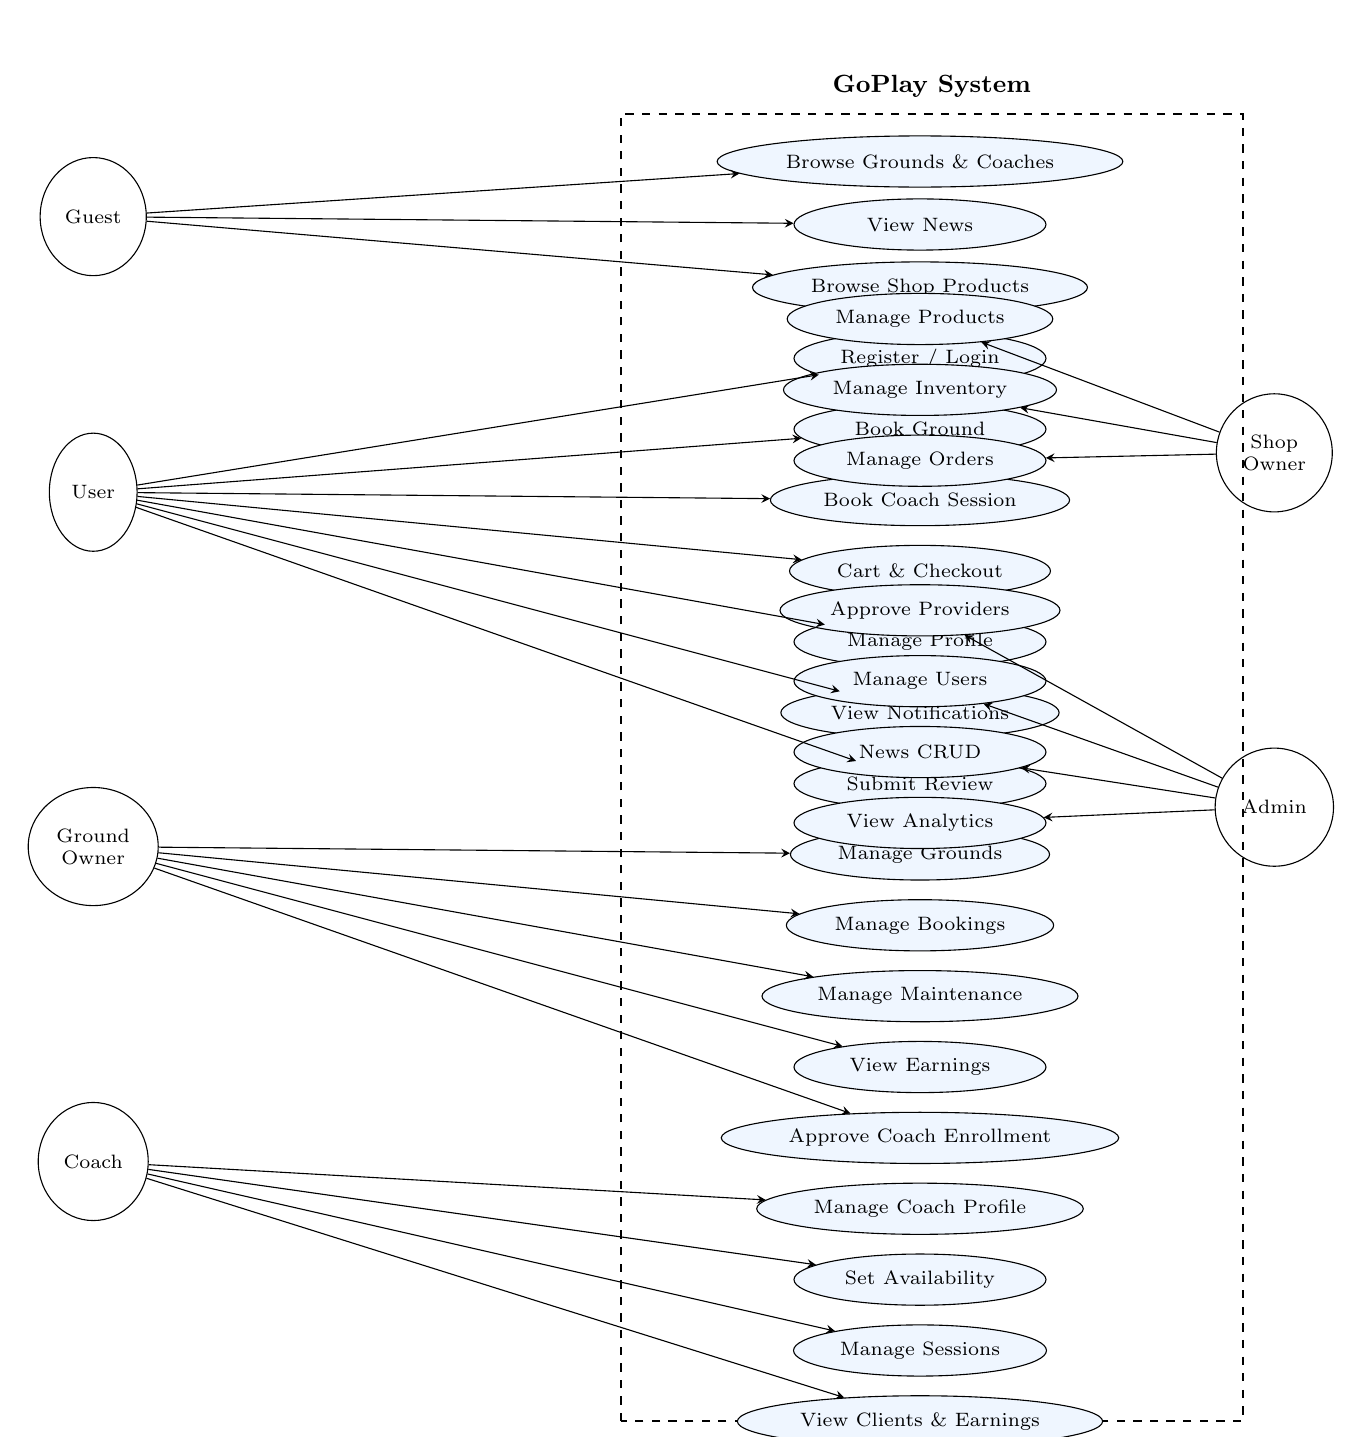
\begin{tikzpicture}[
  actor/.style={draw, ellipse, minimum width=1.1cm, minimum height=1.5cm,
                align=center, font=\scriptsize},
  uc/.style={draw, ellipse, minimum width=3.2cm, minimum height=0.65cm,
             align=center, font=\scriptsize, fill=light},
  arr/.style={->, >=stealth, thin}
]

%% Left actors
\node[actor] (guest)   at (-5.5, 10.5) {Guest};
\node[actor] (user)    at (-5.5,  7.0) {User};
\node[actor] (gowner)  at (-5.5,  2.5) {Ground\\Owner};
\node[actor] (coach)   at (-5.5, -1.5) {Coach};

%% Right actors
\node[actor] (shopown) at ( 9.5,  7.5) {Shop\\Owner};
\node[actor] (admin)   at ( 9.5,  3.0) {Admin};

%% System boundary
\draw[dashed, thick] (1.2, -4.8) rectangle (9.1, 11.8);
\node[font=\small\bfseries] at (5.15, 12.15) {GoPlay System};

%% Guest use cases
\node[uc] (uc_browse)  at (5.0, 11.2) {Browse Grounds \& Coaches};
\node[uc] (uc_viewnews) at (5.0, 10.4) {View News};
\node[uc] (uc_viewshop) at (5.0,  9.6) {Browse Shop Products};

%% User use cases
\node[uc] (uc_reg)    at (5.0,  8.7) {Register / Login};
\node[uc] (uc_bgnd)   at (5.0,  7.8) {Book Ground};
\node[uc] (uc_bcoach) at (5.0,  6.9) {Book Coach Session};
\node[uc] (uc_cart)   at (5.0,  6.0) {Cart \& Checkout};
\node[uc] (uc_prof)   at (5.0,  5.1) {Manage Profile};
\node[uc] (uc_notif)  at (5.0,  4.2) {View Notifications};
\node[uc] (uc_rev)    at (5.0,  3.3) {Submit Review};

%% Ground Owner use cases
\node[uc] (uc_gm)     at (5.0,  2.4) {Manage Grounds};
\node[uc] (uc_bm)     at (5.0,  1.5) {Manage Bookings};
\node[uc] (uc_maint)  at (5.0,  0.6) {Manage Maintenance};
\node[uc] (uc_earn)   at (5.0, -0.3) {View Earnings};
\node[uc] (uc_enroll) at (5.0, -1.2) {Approve Coach Enrollment};

%% Coach use cases
\node[uc] (uc_cp)     at (5.0, -2.1) {Manage Coach Profile};
\node[uc] (uc_avail)  at (5.0, -3.0) {Set Availability};
\node[uc] (uc_sess)   at (5.0, -3.9) {Manage Sessions};
\node[uc] (uc_cli)    at (5.0, -4.8) {View Clients \& Earnings};

%% Shop Owner use cases
\node[uc] (uc_sprod)  at (5.0,  9.2) {Manage Products};
\node[uc] (uc_sinv)   at (5.0,  8.3) {Manage Inventory};
\node[uc] (uc_sord)   at (5.0,  7.4) {Manage Orders};

%% Admin use cases
\node[uc] (uc_apps)   at (5.0,  5.5) {Approve Providers};
\node[uc] (uc_umgmt)  at (5.0,  4.6) {Manage Users};
\node[uc] (uc_news)   at (5.0,  3.7) {News CRUD};
\node[uc] (uc_anal)   at (5.0,  2.8) {View Analytics};

%% Guest arrows
\draw[arr] (guest) -- (uc_browse);
\draw[arr] (guest) -- (uc_viewnews);
\draw[arr] (guest) -- (uc_viewshop);

%% User arrows
\draw[arr] (user) -- (uc_reg);
\draw[arr] (user) -- (uc_bgnd);
\draw[arr] (user) -- (uc_bcoach);
\draw[arr] (user) -- (uc_cart);
\draw[arr] (user) -- (uc_prof);
\draw[arr] (user) -- (uc_notif);
\draw[arr] (user) -- (uc_rev);

%% Ground Owner arrows
\draw[arr] (gowner) -- (uc_gm);
\draw[arr] (gowner) -- (uc_bm);
\draw[arr] (gowner) -- (uc_maint);
\draw[arr] (gowner) -- (uc_earn);
\draw[arr] (gowner) -- (uc_enroll);

%% Coach arrows
\draw[arr] (coach) -- (uc_cp);
\draw[arr] (coach) -- (uc_avail);
\draw[arr] (coach) -- (uc_sess);
\draw[arr] (coach) -- (uc_cli);

%% Shop Owner arrows
\draw[arr] (shopown) -- (uc_sprod);
\draw[arr] (shopown) -- (uc_sinv);
\draw[arr] (shopown) -- (uc_sord);

%% Admin arrows
\draw[arr] (admin) -- (uc_apps);
\draw[arr] (admin) -- (uc_umgmt);
\draw[arr] (admin) -- (uc_news);
\draw[arr] (admin) -- (uc_anal);

\end{tikzpicture}
\caption{GoPlay Use Case Diagram}
\label{fig:usecase}
\end{figure}

\section{Class Diagram}

\begin{figure}[H]
\centering
\begin{tikzpicture}[
  cls/.style={draw, rectangle, minimum width=3cm, font=\scriptsize, align=left},
  arr/.style={->, >=stealth},
  scale=0.95, transform shape
]
\node[cls] (user) at (0,0) {
  \textbf{User}\\[-2pt]\hline
  id, email, password\_hash\\
  user\_type, first\_name\\
  profile\_picture, status\\[-2pt]\hline
  find(), update()\\
  verifyPassword()\\
  getStatistics()
};
\node[cls] (coach) at (5.5,0) {
  \textbf{Coach}\\[-2pt]\hline
  id, user\_id, bio\\
  sport\_category\_id\\
  hourly\_rate\\[-2pt]\hline
  getByUserId()\\
  getCertificates()\\
  getFacilities()
};
\node[cls] (cbooking) at (5.5,-4) {
  \textbf{CoachBooking}\\[-2pt]\hline
  id, coach\_id, user\_id\\
  booking\_date\\
  start\_time, end\_time\\
  status, total\_amount\\[-2pt]\hline
  create(), cancel()\\
  getEarningsStats()
};
\node[cls] (facility) at (0,-4) {
  \textbf{SportsFacility}\\[-2pt]\hline
  id, owner\_user\_id\\
  name, location\\
  sport\_id, hourly\_rate\\[-2pt]\hline
  create(), update()\\
  getLinkedCoaches()
};
\node[cls] (gbooking) at (-5.5,-4) {
  \textbf{GroundBooking}\\[-2pt]\hline
  id, facility\_id\\
  user\_id, booking\_date\\
  start\_time, end\_time\\
  total\_price, status\\[-2pt]\hline
  create(), cancel()
};
\node[cls] (product) at (-5.5,0) {
  \textbf{Product}\\[-2pt]\hline
  id, shop\_owner\_id\\
  name, price\\
  stock\_qty, category\_id\\[-2pt]\hline
  create(), update()\\
  getLowStock()
};
\node[cls] (order) at (-5.5,-8) {
  \textbf{Order}\\[-2pt]\hline
  id, user\_id\\
  total\_amount, status\\
  payment\_method\\[-2pt]\hline
  createOrder()\\
  updateStatus()
};
\node[cls] (news) at (5.5,-8) {
  \textbf{News}\\[-2pt]\hline
  id, title, slug\\
  category, status\\
  featured, view\_count\\[-2pt]\hline
  getPublished()\\
  getFeatured()\\
  getTrending()
};
\node[cls] (review) at (0,-8) {
  \textbf{FacilityReview}\\[-2pt]\hline
  id, facility\_id\\
  user\_id, rating\\
  comment, reply\\[-2pt]\hline
  saveReply()\\
  reportReview()
};

%% Relationships
\draw[arr] (coach.west) -- node[above]{\tiny user\_id} (user.east);
\draw[arr] (cbooking.north) -- node[right]{\tiny coach\_id} (coach.south);
\draw[arr] (cbooking) -- node[above]{\tiny user\_id} (user);
\draw[arr] (gbooking.north) -- node[left]{\tiny facility\_id} (facility.south);
\draw[arr] (gbooking.east) -- node[above]{\tiny user\_id} (user.west);
\draw[arr] (facility.west) -- node[above]{\tiny owner} (user.east);
\draw[arr] (product.east) -- node[above]{\tiny shop\_owner\_id} (user.west);
\draw[arr] (order.north) -- node[left]{\tiny user\_id} (gbooking.south);
\draw[arr] (review.west) -- node[below]{\tiny facility\_id} (facility.south);
\end{tikzpicture}
\caption{GoPlay Simplified Class Diagram (Key Models)}
\label{fig:class}
\end{figure}

\section{Entity-Relationship (ER) Diagram}

The platform uses 50+ database tables. The table below lists the key entities and their relationships. A complete ER diagram should be generated from \texttt{database/schema.sql} using a tool such as MySQL Workbench or draw.io.

\begin{center}
\begin{longtable}{p{4.5cm} p{4cm} p{5.5cm}}
\toprule
\textbf{Entity / Table} & \textbf{Key Attributes} & \textbf{Relationships}\\
\midrule
\endhead
users                  & id, email, user\_type, status           & 1 user $\to$ many bookings, orders\\
coaches                & id, user\_id, sport\_id, hourly\_rate   & 1 coach $\to$ 1 user; many sessions\\
sports\_facilities     & id, owner\_user\_id, sport\_id          & 1 facility $\to$ many bookings, reviews\\
facility\_bookings     & id, facility\_id, user\_id              & M:M facilities and users\\
coach\_bookings        & id, coach\_id, user\_id                 & M:M coaches and users\\
coach\_facilities      & coach\_id, facility\_id, status         & M:M coaches and facilities\\
facility\_reviews      & id, facility\_id, user\_id              & 1 facility $\to$ many reviews\\
facility\_review\_reports & id, review\_id, user\_id             & 1 review $\to$ many reports\\
coach\_certificates    & id, coach\_id                           & 1 coach $\to$ many certs\\
coach\_achievements    & id, coach\_id                           & 1 coach $\to$ many achievements\\
facility\_maintenance\_tasks & id, facility\_id                  & 1 facility $\to$ many tasks\\
facility\_inspections  & id, facility\_id                        & 1 facility $\to$ many inspections\\
products               & id, shop\_owner\_id, category\_id       & 1 shop owner $\to$ many products\\
product\_reviews       & id, product\_id, user\_id               & 1 product $\to$ many reviews\\
shopping\_cart         & id, user\_id / session\_id              & 1 user/guest $\to$ 1 cart\\
cart\_items            & id, cart\_id, product\_id               & M:M carts and products\\
orders                 & id, user\_id, total\_amount             & 1 user $\to$ many orders\\
order\_items           & id, order\_id, product\_id              & M:M orders and products\\
payments               & id, order/booking ref                   & 1 payment $\to$ 1 order/booking\\
payhere\_transactions  & id, transaction\_id                     & 1 transaction $\to$ 1 payment\\
platform\_earnings     & id, booking/order ref                   & Service fee per transaction\\
withdrawal\_requests   & id, user\_id, amount, status            & 1 provider $\to$ many requests\\
provider\_applications & id, user\_id, type, status              & 1 user $\to$ 1 application\\
news                   & id, title, slug, category, featured     & Standalone; admin managed\\
notifications          & id, user\_id, type, message             & 1 user $\to$ many notifications\\
user\_activity\_log    & id, user\_id, action                    & 1 user $\to$ many log entries\\
admin\_logs            & id, admin\_id, action                   & 1 admin $\to$ many log entries\\
settings               & key, value                              & System configuration\\
\bottomrule
\end{longtable}
\end{center}

\section{Activity Diagrams}

\subsection{Ground Booking Activity Diagram}

\begin{figure}[H]
\centering
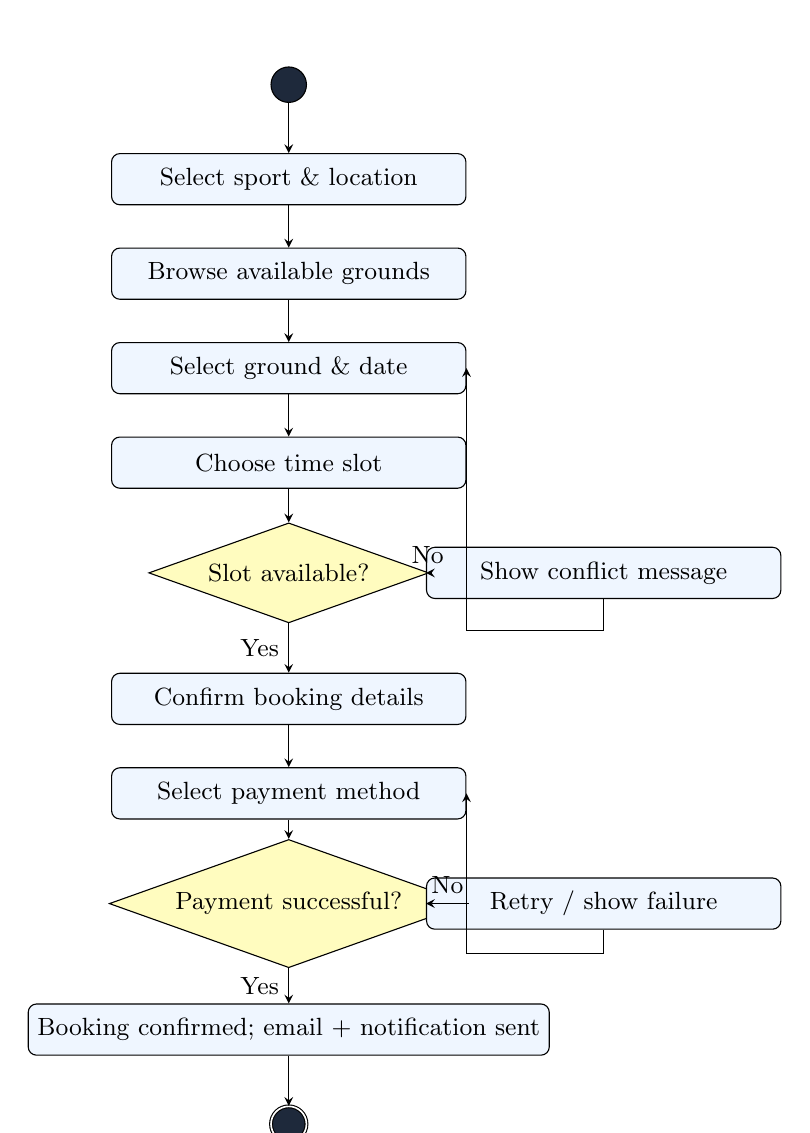
\begin{tikzpicture}[
  start/.style={draw,circle,fill=dark,minimum size=0.45cm},
  endd/.style={draw,circle,fill=dark,minimum size=0.45cm,double},
  act/.style={draw,rectangle,rounded corners=3pt,minimum width=4.5cm,
              minimum height=0.65cm,align=center,font=\small,fill=light},
  dec/.style={draw,diamond,aspect=2.8,align=center,font=\small,fill=yellow!25},
  arr/.style={->,>=stealth}
]
\node[start] (s) at (0,0) {};
\node[act]   (a1) at (0,-1.2) {Select sport \& location};
\node[act]   (a2) at (0,-2.4) {Browse available grounds};
\node[act]   (a3) at (0,-3.6) {Select ground \& date};
\node[act]   (a4) at (0,-4.8) {Choose time slot};
\node[dec]   (d1) at (0,-6.2) {Slot available?};
\node[act]   (a5) at (4,-6.2) {Show conflict message};
\node[act]   (a6) at (0,-7.8) {Confirm booking details};
\node[act]   (a7) at (0,-9.0) {Select payment method};
\node[dec]   (d2) at (0,-10.4){Payment successful?};
\node[act]   (a8) at (4,-10.4){Retry / show failure};
\node[act]   (a9) at (0,-12.0){Booking confirmed; email + notification sent};
\node[endd]  (e)  at (0,-13.2){};

\draw[arr] (s)--(a1);
\draw[arr] (a1)--(a2);
\draw[arr] (a2)--(a3);
\draw[arr] (a3)--(a4);
\draw[arr] (a4)--(d1);
\draw[arr] (d1)--node[above]{\small No}(a5);
\draw[arr] (d1)--node[left]{\small Yes}(a6);
\draw[arr] (a5.south)--++(0,-0.4)-|(a3.east);
\draw[arr] (a6)--(a7);
\draw[arr] (a7)--(d2);
\draw[arr] (d2)--node[above]{\small No}(a8);
\draw[arr] (d2)--node[left]{\small Yes}(a9);
\draw[arr] (a8.south)--++(0,-0.3)-|(a7.east);
\draw[arr] (a9)--(e);
\end{tikzpicture}
\caption{Activity Diagram -- Ground Booking Process}
\label{fig:act_booking}
\end{figure}

\subsection{Provider Application and Approval Activity Diagram}

\begin{figure}[H]
\centering
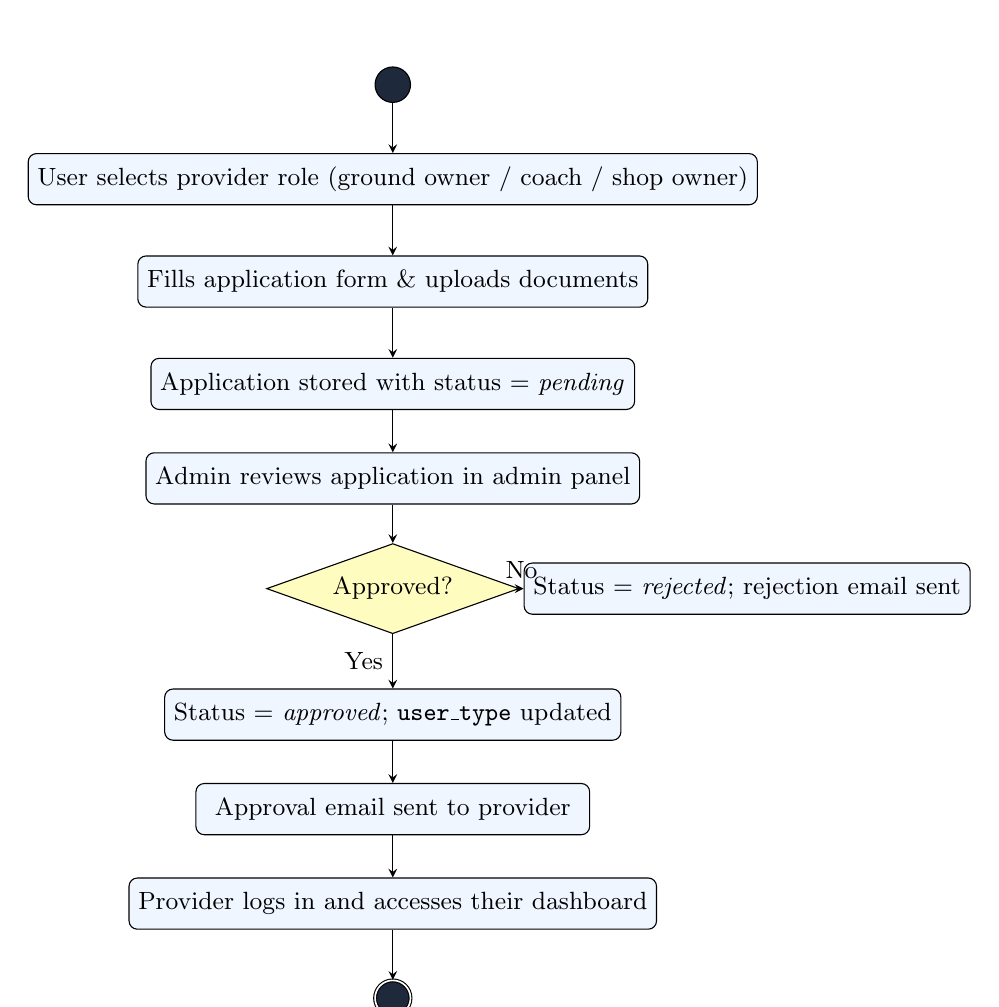
\begin{tikzpicture}[
  start/.style={draw,circle,fill=dark,minimum size=0.45cm},
  endd/.style={draw,circle,fill=dark,minimum size=0.45cm,double},
  act/.style={draw,rectangle,rounded corners=3pt,minimum width=5cm,
              minimum height=0.65cm,align=center,font=\small,fill=light},
  dec/.style={draw,diamond,aspect=2.8,align=center,font=\small,fill=yellow!25},
  arr/.style={->,>=stealth}
]
\node[start] (s)  at (0,0) {};
\node[act]   (a1) at (0,-1.2) {User selects provider role (ground owner / coach / shop owner)};
\node[act]   (a2) at (0,-2.5) {Fills application form \& uploads documents};
\node[act]   (a3) at (0,-3.8) {Application stored with status = \textit{pending}};
\node[act]   (a4) at (0,-5.0) {Admin reviews application in admin panel};
\node[dec]   (d1) at (0,-6.4) {Approved?};
\node[act]   (a5) at (4.5,-6.4){Status = \textit{rejected}; rejection email sent};
\node[act]   (a6) at (0,-8.0) {Status = \textit{approved}; \texttt{user\_type} updated};
\node[act]   (a7) at (0,-9.2) {Approval email sent to provider};
\node[act]   (a8) at (0,-10.4){Provider logs in and accesses their dashboard};
\node[endd]  (e)  at (0,-11.6){};

\draw[arr] (s)--(a1);
\draw[arr] (a1)--(a2);
\draw[arr] (a2)--(a3);
\draw[arr] (a3)--(a4);
\draw[arr] (a4)--(d1);
\draw[arr] (d1)--node[above]{\small No}(a5);
\draw[arr] (d1)--node[left]{\small Yes}(a6);
\draw[arr] (a6)--(a7);
\draw[arr] (a7)--(a8);
\draw[arr] (a8)--(e);
\end{tikzpicture}
\caption{Activity Diagram -- Provider Application Process}
\label{fig:act_provider}
\end{figure}

%% =============================================================================
\chapter{Completeness of the Project}
%% =============================================================================

\section{Functionalities Completed}

\subsection{User Module (Malika Nishnatha)}

\begin{itemize}[leftmargin=1.5cm]
  \item User registration with automatic username generation, login, logout, and session management.
  \item User dashboard displaying ground booking count, coach session count, order count, and activity statistics.
  \item Browse and search sports grounds by sport type and location with real-time availability display.
  \item Ground slot booking with date/time selection, availability validation, and booking record creation.
  \item Multi-step checkout: contact details $\to$ payment method $\to$ PayHere gateway / COD / card $\to$ order confirmation.
  \item Shopping cart with guest support and session-to-user merge on login (add, update quantity, remove, clear).
  \item Order history with per-order item breakdown and order status tracking.
  \item Coach session booking from the user side (browse coaches, view public profile, select available slot, book).
  \item My Coach Sessions page (view upcoming and past sessions, reschedule, cancel).
  \item My Bookings page for ground facility reservations with status display.
  \item User profile management: update personal info, upload avatar, change password (Argon2id hashed).
  \item In-app notification centre with read/unread state and notification type icons.
  \item User account settings page.
  \item Facility review submission with star rating and text comment.
  \item Login history recorded with timestamp, IP address, and user-agent string.
  \item User activity logged for audit purposes.
\end{itemize}

\subsection{Ground Owner Module (Malika Nishnatha)}

\begin{itemize}[leftmargin=1.5cm]
  \item Ground owner provider application with document upload and admin approval workflow.
  \item Ground owner dashboard with facility count, booking statistics, and revenue overview.
  \item Sports facility CRUD: create, update, and delete facility listings with images and sport type.
  \item Facility availability configuration: set weekly opening hours and block specific dates.
  \item Booking dashboard: view all facility bookings with status filters (pending, confirmed, completed, cancelled).
  \item Weekly schedule view of all upcoming bookings across all owned facilities.
  \item Ground owner earnings dashboard with period-based breakdown (daily, weekly, monthly) and per-facility breakdown.
  \item Maintenance task management: create tasks, assign categories, update progress, mark complete, track cost trends.
  \item Facility inspection management: schedule inspections, record results and health scores, track overdue inspections.
  \item Facility review management: inline reply (upsert reply), delete reply, and report inappropriate reviews.
  \item Coach enrollment management: view pending/approved/rejected coach link requests, approve or reject with notification to coach.
  \item Ground owner notifications centre.
  \item Ground owner profile page (personal info, business details, bio).
  \item Ground owner account settings.
\end{itemize}

\subsection{Coach Module (Winuka Mahagamage)}

\begin{itemize}[leftmargin=1.5cm]
  \item Coach provider application and admin approval workflow.
  \item Coach dashboard with session count, client count, earnings overview, and recent activity.
  \item Professional profile management: bio, sport specialisation, experience years, hourly rate, avatar upload.
  \item Certificates CRUD: add, edit, delete professional certifications with issuer name, issue date, and description.
  \item Achievements CRUD: add, edit, delete awards and accomplishments with category, date, and description.
  \item Weekly availability schedule editor: per-day on/off toggles with start and end time pickers; saved to \texttt{coach\_availability} table.
  \item Monthly booking calendar view with booked-date badges.
  \item Upcoming sessions list sorted by date.
  \item Session management: view all sessions; confirm, mark as complete, or cancel; status tracked from \texttt{pending} to \texttt{completed} / \texttt{no-show}.
  \item Client management dashboard: grid and list view of clients with total sessions, spending, and last session date; per-client booking history modal; CSV data export.
  \item Coach earnings dashboard: per-session income breakdown, total earnings, period trends, all in LKR.
  \item Review management: view all user reviews with star ratings; reply to reviews; responses stored as replies.
  \item Facility connection: link to multiple sports facilities (creates \texttt{coach\_facilities} record with \texttt{pending} status); set primary facility; unlink facility.
  \item Public coach profile page: displays bio, credentials, achievements, linked facilities, and available time slots for user booking.
  \item Bundled booking: user books coach session + linked facility slot in a single atomic database transaction.
  \item Coach appears on facility's coaches sidebar once enrollment is approved by the ground owner.
\end{itemize}

\subsection{Admin Module (Ravindu)}

\begin{itemize}[leftmargin=1.5cm]
  \item Admin dashboard with platform-wide KPI cards (total users, total bookings, total revenue, active providers).
  \item Provider application management: list all applications (ground owner, coach, shop owner) with search, status filter, and type filter; view full application detail including uploaded documents; approve or reject with automated email notification.
  \item User management (\texttt{AdminUserController}): list users with role and status filters; view user details; update user role and status; reset passwords; delete accounts; view user statistics.
  \item Platform payment and earnings management (\texttt{AdminPaymentController}): view all payment transactions; configure service fee percentages; process and track provider withdrawal requests; revenue analytics.
  \item Full analytics dashboard (\texttt{AnalyticsController}): user growth trends; revenue over time; booking activity (ground and coach); product sales performance; platform activity logs; data export capability.
  \item System settings management: update configuration values in bulk; test email delivery; trigger database backup; clear cache.
  \item News article CRUD (\texttt{AdminNewsController}): create, edit, publish/unpublish, and delete articles; assign categories (Cricket, Football, Basketball, Tennis, Swimming, General Sports); mark articles as featured; manage news thumbnails.
  \item Public news listing: paginated article list with category filter tabs, keyword search, live search API, and hero section featuring the latest featured article.
  \item News detail page: full article view with formatted content, view-count increment on each visit, and related articles section.
  \item Trending news based on view counts.
  \item All admin actions logged in \texttt{admin\_logs} with admin ID, action type, and timestamp for full auditability.
\end{itemize}

\subsection{Shop Owner Module (Piyumi)}

\begin{itemize}[leftmargin=1.5cm]
  \item Shop owner provider application and admin approval workflow.
  \item Shop owner dashboard: total products, active products, low-stock count, total orders, pending/processing/shipped/delivered order counts, total revenue, monthly revenue, recent orders, top-selling products, low-stock product alerts, and recent reviews.
  \item Product management CRUD: add, edit, and delete products with name, description, price, category, stock quantity, and image upload.
  \item Product category management with item count display.
  \item Inventory management page: list all products with stock levels; edit minimum stock thresholds; trigger low-stock alerts on dashboard.
  \item Order management: list all orders with status filters; update order status through the lifecycle (pending $\to$ processing $\to$ shipped $\to$ delivered); view per-order item details.
  \item Product review management: view all customer reviews with star ratings and comments; read review replies.
  \item Shop owner profile management: update business information, tax details, delivery options; upload shop logo, banner image, and business registration documents.
  \item Public shop page (\texttt{ProductController}): product grid with category filters, price sorting, and keyword search; product detail page with images, description, and review section; review submission by verified buyers.
\end{itemize}

\section{Functionalities Yet to Complete}

\begin{itemize}[leftmargin=1.5cm]
  \item \textbf{Password Reset via Email:} Forgot-password / OTP email flow is not yet implemented. Users who forget their password cannot self-reset without admin intervention.
  \item \textbf{Automated Refund Processing:} Cancelling a paid booking updates the status but does not programmatically trigger a PayHere refund. Refunds must be handled manually.
  \item \textbf{Admin Analytics Charts:} The analytics dashboard serves data via API but time-series charts (booking trends, revenue over time) are placeholder containers not yet connected to a charting library.
  \item \textbf{Coach Review System (User-Facing):} A \texttt{coach\_reviews} table and model exist, but the user-facing UI to submit a review after a completed coach session has not been surfaced.
  \item \textbf{Multi-Image Product Gallery:} Products currently support a single image. The \texttt{product\_images} table is defined but multi-image upload on the shop owner side is not fully implemented.
  \item \textbf{Withdrawal Approval UI:} Ground owners and coaches can submit withdrawal requests (stored in \texttt{withdrawal\_requests}), but the admin-side approval, payout confirmation, and rejection flow is not fully built.
  \item \textbf{Advanced Ground Search Filters:} Currently filters by sport type and location only. Price-range, rating, amenities, and distance filters are not yet available.
  \item \textbf{Notification Email Completeness:} PHPMailer is integrated; booking confirmation and provider approval emails are sent. However, order status change emails and review notification emails are not yet wired up.
  \item \textbf{Mobile Optimisation:} Core layouts are responsive, but some standalone provider dashboard pages (coach earnings, ground owner maintenance) require further responsive breakpoint tuning for smaller screens.
\end{itemize}

\section{Individual Contribution}

\subsection{Malika Nishnatha --- User Module \& Ground Owner Module (30\%)}

\textbf{Completed Functionalities:}

\textit{User Module}
\begin{itemize}[leftmargin=1.5cm]
  \item \textbf{Authentication \& Session:} User registration with automatic username generation; secure login and logout; session management using \texttt{startSession()}.
  \item \textbf{Dashboard:} Personalised dashboard displaying ground booking count, coach session count, order count, and recent activity statistics.
  \item \textbf{Ground Booking:} Browse and search sports facilities by sport type and location; real-time slot availability checking; date and time slot selection; booking record creation with status tracking.
  \item \textbf{Coach Sessions:} Browse coaches, view public coach profile, select an available slot, and book a session; My Coach Sessions page for viewing, rescheduling, and cancelling sessions.
  \item \textbf{Shopping \& Checkout:} Persistent shopping cart with guest support and session-to-user merge on login; multi-step checkout (contact details $\to$ payment method $\to$ PayHere / COD / card $\to$ confirmation); order history with per-order item breakdown.
  \item \textbf{Profile \& Account:} Update personal information; upload avatar (Argon2id-hashed password change); account settings page.
  \item \textbf{Notifications \& Audit:} In-app notification centre with read/unread state; login history recorded with IP and user-agent; user activity logged for audit purposes; facility review submission with star rating and comment.
\end{itemize}

\textit{Ground Owner Module}
\begin{itemize}[leftmargin=1.5cm]
  \item \textbf{Application Workflow:} Provider application with document upload; admin approval/rejection with email notification.
  \item \textbf{Facility Management:} Create, update, and delete sports facility listings with images and sport type; dashboard with facility count, booking statistics, and revenue overview.
  \item \textbf{Booking \& Availability:} View and filter all facility bookings by status; weekly schedule view across all owned facilities; configure weekly opening hours and block specific dates.
  \item \textbf{Earnings Dashboard:} Period-based earnings breakdown (daily, weekly, monthly) with per-facility breakdown.
  \item \textbf{Maintenance \& Inspections:} Create and track maintenance tasks with categories, progress notes, and cost trends; schedule facility safety inspections, record results and health scores, track overdue inspections.
  \item \textbf{Reviews \& Coach Enrollment:} Inline reply and delete reply on facility reviews; report inappropriate reviews; view and approve or reject coach enrollment requests with notification to coach.
  \item \textbf{Profile \& Notifications:} Ground owner profile page (personal info, business details, bio); notifications centre; account settings.
\end{itemize}

\textbf{Test Cases:}

\textit{User Authentication}

\begin{center}
\footnotesize
\begin{longtable}{p{0.4cm} p{2.2cm} p{1.8cm} p{3.2cm} p{2.2cm} p{2.2cm} p{1.4cm} p{0.8cm}}
\toprule
\textbf{ID} & \textbf{Description} & \textbf{Precondition} & \textbf{Test Steps} & \textbf{Test Data} & \textbf{Expected} & \textbf{Actual} & \textbf{P/F}\\
\midrule
\endhead
1 & Register a new user & Email not already registered & Navigate to register page $\to$ fill first name, last name, email, password $\to$ click register & Name: Test User, email: newuser@gmail.com, password: Test@1234 & Session created, user redirected to dashboard & As expected & Pass\\[4pt]
2 & Login with incorrect password & User account exists & Navigate to login $\to$ enter email $\to$ enter incorrect password $\to$ click sign-in & email: user@gmail.com, password: wrongpass & Error message shown, session not created & As expected & Pass\\
\bottomrule
\end{longtable}
\end{center}

\textit{Ground Browsing \& Booking}

\begin{center}
\footnotesize
\begin{longtable}{p{0.4cm} p{2.2cm} p{1.8cm} p{3.2cm} p{2.2cm} p{2.2cm} p{1.4cm} p{0.8cm}}
\toprule
\textbf{ID} & \textbf{Description} & \textbf{Precondition} & \textbf{Test Steps} & \textbf{Test Data} & \textbf{Expected} & \textbf{Actual} & \textbf{P/F}\\
\midrule
\endhead
3 & Search grounds by sport & Football facilities exist in DB & Go to grounds page $\to$ select sport ``Football'' $\to$ submit search & Sport: Football & Only football facilities returned in results & As expected & Pass\\[4pt]
4 & Book an available slot & User logged in, slot available & Select ground $\to$ choose date $\to$ choose available time slot $\to$ confirm booking & Date: 2026-04-20, time: 10:00--12:00 & \texttt{facility\_bookings} record created with status \texttt{pending} & As expected & Pass\\[4pt]
5 & Attempt duplicate booking & Same slot already booked & Select same ground $\to$ same date $\to$ same time slot $\to$ attempt booking & Same date/time as existing booking & Conflict error returned, no duplicate record created & As expected & Pass\\
\bottomrule
\end{longtable}
\end{center}

\textit{Shopping Cart \& Checkout}

\begin{center}
\footnotesize
\begin{longtable}{p{0.4cm} p{2.2cm} p{1.8cm} p{3.2cm} p{2.2cm} p{2.2cm} p{1.4cm} p{0.8cm}}
\toprule
\textbf{ID} & \textbf{Description} & \textbf{Precondition} & \textbf{Test Steps} & \textbf{Test Data} & \textbf{Expected} & \textbf{Actual} & \textbf{P/F}\\
\midrule
\endhead
6 & Add two products and update quantity & User logged in, products exist & Add product A to cart $\to$ add product B $\to$ update product A quantity $\to$ view cart & Product A qty: 1$\to$2, Product B qty: 1 & Cart totals update correctly & As expected & Pass\\[4pt]
7 & Complete checkout via PayHere sandbox & Items in cart, user logged in & Go to checkout $\to$ enter contact details $\to$ select PayHere $\to$ complete sandbox payment & PayHere sandbox credentials & \texttt{orders} and \texttt{payments} records created in DB & As expected & Pass\\
\bottomrule
\end{longtable}
\end{center}

\textit{Profile Management}

\begin{center}
\footnotesize
\begin{longtable}{p{0.4cm} p{2.2cm} p{1.8cm} p{3.2cm} p{2.2cm} p{2.2cm} p{1.4cm} p{0.8cm}}
\toprule
\textbf{ID} & \textbf{Description} & \textbf{Precondition} & \textbf{Test Steps} & \textbf{Test Data} & \textbf{Expected} & \textbf{Actual} & \textbf{P/F}\\
\midrule
\endhead
8 & Upload a new avatar & User logged in & Go to profile $\to$ click upload avatar $\to$ select image file $\to$ save changes & JPG image file ($<$2 MB) & File saved on server, \texttt{users.profile\_picture} updated & As expected & Pass\\
\bottomrule
\end{longtable}
\end{center}

\textit{Ground Owner -- Facility Management}

\begin{center}
\footnotesize
\begin{longtable}{p{0.4cm} p{2.2cm} p{1.8cm} p{3.2cm} p{2.2cm} p{2.2cm} p{1.4cm} p{0.8cm}}
\toprule
\textbf{ID} & \textbf{Description} & \textbf{Precondition} & \textbf{Test Steps} & \textbf{Test Data} & \textbf{Expected} & \textbf{Actual} & \textbf{P/F}\\
\midrule
\endhead
9 & Ground owner creates a new facility & Ground owner approved and logged in & Go to facilities $\to$ click add facility $\to$ fill name, sport, city, price $\to$ save & Name: City Ground, sport: Cricket, city: Colombo, rate: LKR~3,000/hr & Facility appears on the public ground browsing page & As expected & Pass\\[4pt]
10 & Ground owner blocks a date & Ground owner has a facility & Go to availability $\to$ select facility $\to$ pick date to block $\to$ save & Date: 2026-04-25 & Date shows as unavailable to users attempting to book & As expected & Pass\\
\bottomrule
\end{longtable}
\end{center}

\textit{Ground Owner -- Operations}

\begin{center}
\footnotesize
\begin{longtable}{p{0.4cm} p{2.2cm} p{1.8cm} p{3.2cm} p{2.2cm} p{2.2cm} p{1.4cm} p{0.8cm}}
\toprule
\textbf{ID} & \textbf{Description} & \textbf{Precondition} & \textbf{Test Steps} & \textbf{Test Data} & \textbf{Expected} & \textbf{Actual} & \textbf{P/F}\\
\midrule
\endhead
11 & Create maintenance task & Ground owner logged in, facility exists & Go to maintenance $\to$ click add task $\to$ fill title, category, description $\to$ save & Task: Fix boundary nets, category: Equipment & Task appears in maintenance list with status \texttt{pending} & As expected & Pass\\[4pt]
12 & Approve coach enrollment request & Coach has requested link to facility & Go to coaches $\to$ find pending request $\to$ click approve $\to$ confirm & -- & \texttt{coach\_facilities.status} = \texttt{approved}, coach notification created & As expected & Pass\\[4pt]
13 & Reply to a facility review & Review exists on facility & Go to reviews $\to$ find review $\to$ click reply $\to$ type response $\to$ save & Reply: ``Thank you for your feedback!'' & Reply saved and displayed under the review & As expected & Pass\\
\bottomrule
\end{longtable}
\end{center}

\subsection{Winuka Mahagamage --- Coach Module (25\%)}

\textbf{Completed Functionalities:}

\begin{itemize}[leftmargin=1.5cm]
  \item \textbf{Application \& Dashboard:} Coach provider application and admin approval workflow; coach dashboard with session count, client count, earnings overview, and recent activity.
  \item \textbf{Professional Profile:} Manage bio, sport specialisation, experience years, hourly rate, and avatar upload.
  \item \textbf{Certificates \& Achievements:} Full CRUD for professional certificates (name, issuer, date, description) and achievements (title, category, date, description).
  \item \textbf{Availability Management:} Weekly schedule editor with per-day on/off toggles and start/end time pickers; monthly booking calendar view with booked-date badges; upcoming sessions list sorted by date.
  \item \textbf{Session Management:} View all sessions; confirm, mark as complete, or cancel; status tracked from \texttt{pending} through \texttt{completed} / \texttt{no-show}.
  \item \textbf{Client Management:} Grid and list view of clients with total sessions, total spending, and last session date; per-client booking history modal; CSV data export.
  \item \textbf{Earnings Dashboard:} Per-session income breakdown, total earnings, and period trends displayed in LKR.
  \item \textbf{Review Management:} View all user reviews with star ratings; write and save replies to reviews.
  \item \textbf{Facility Linking:} Request links to sports facilities (\texttt{pending} $\to$ \texttt{approved}); set a primary facility; unlink a facility; status badges shown per link.
  \item \textbf{Public Profile \& Bundled Booking:} Public coach profile page displaying bio, credentials, achievements, linked facilities, and available time slots; bundled coach + facility booking in a single atomic database transaction.
\end{itemize}

\textbf{Test Cases:}

\textit{Coach Profile \& Certificates}

\begin{center}
\footnotesize
\begin{longtable}{p{0.4cm} p{2.2cm} p{1.8cm} p{3.2cm} p{2.2cm} p{2.2cm} p{1.4cm} p{0.8cm}}
\toprule
\textbf{ID} & \textbf{Description} & \textbf{Precondition} & \textbf{Test Steps} & \textbf{Test Data} & \textbf{Expected} & \textbf{Actual} & \textbf{P/F}\\
\midrule
\endhead
1 & Coach adds a certificate & Coach logged in & Go to profile $\to$ certificates tab $\to$ click add $\to$ fill name, issuer, date, description $\to$ save & Cert: Tennis Level 2, issuer: LTA, date: 2024-01-15 & Certificate appears on the public coach profile page & As expected & Pass\\
\bottomrule
\end{longtable}
\end{center}

\textit{Availability}

\begin{center}
\footnotesize
\begin{longtable}{p{0.4cm} p{2.2cm} p{1.8cm} p{3.2cm} p{2.2cm} p{2.2cm} p{1.4cm} p{0.8cm}}
\toprule
\textbf{ID} & \textbf{Description} & \textbf{Precondition} & \textbf{Test Steps} & \textbf{Test Data} & \textbf{Expected} & \textbf{Actual} & \textbf{P/F}\\
\midrule
\endhead
2 & Set Monday availability & Coach logged in & Go to availability $\to$ toggle Monday on $\to$ set start 09:00, end 17:00 $\to$ save & Day: Monday, start: 09:00, end: 17:00 & Monday time slots appear on the booking page & As expected & Pass\\
\bottomrule
\end{longtable}
\end{center}

\textit{Session Management}

\begin{center}
\footnotesize
\begin{longtable}{p{0.4cm} p{2.2cm} p{1.8cm} p{3.2cm} p{2.2cm} p{2.2cm} p{1.4cm} p{0.8cm}}
\toprule
\textbf{ID} & \textbf{Description} & \textbf{Precondition} & \textbf{Test Steps} & \textbf{Test Data} & \textbf{Expected} & \textbf{Actual} & \textbf{P/F}\\
\midrule
\endhead
3 & User books a coach session & Coach has availability, user logged in & Browse coaches $\to$ open coach profile $\to$ select date $\to$ select slot $\to$ fill details $\to$ submit & Date: 2026-04-21, slot: 10:00--11:00 & Session appears in coach's upcoming sessions list & As expected & Pass\\[4pt]
4 & Coach marks session as complete & Session status is confirmed & Go to sessions $\to$ find session $\to$ click ``Mark Complete'' $\to$ confirm & -- & Status updated to \texttt{completed}, earnings record created & As expected & Pass\\
\bottomrule
\end{longtable}
\end{center}

\textit{Facility Linking}

\begin{center}
\footnotesize
\begin{longtable}{p{0.4cm} p{2.2cm} p{1.8cm} p{3.2cm} p{2.2cm} p{2.2cm} p{1.4cm} p{0.8cm}}
\toprule
\textbf{ID} & \textbf{Description} & \textbf{Precondition} & \textbf{Test Steps} & \textbf{Test Data} & \textbf{Expected} & \textbf{Actual} & \textbf{P/F}\\
\midrule
\endhead
5 & Coach requests facility link & Coach logged in, facility exists & Go to profile $\to$ facilities tab $\to$ click add $\to$ select facility $\to$ submit request & Facility: City Sports Ground, Colombo & \texttt{coach\_facilities} record created with status \texttt{pending}, ground owner notification sent & As expected & Pass\\[4pt]
6 & Ground owner approves link & Link request is pending & Ground owner goes to coaches $\to$ find pending request $\to$ click approve $\to$ confirm & -- & Coach appears on facility's coaches sidebar & As expected & Pass\\
\bottomrule
\end{longtable}
\end{center}

\textit{Bundled Booking}

\begin{center}
\footnotesize
\begin{longtable}{p{0.4cm} p{2.2cm} p{1.8cm} p{3.2cm} p{2.2cm} p{2.2cm} p{1.4cm} p{0.8cm}}
\toprule
\textbf{ID} & \textbf{Description} & \textbf{Precondition} & \textbf{Test Steps} & \textbf{Test Data} & \textbf{Expected} & \textbf{Actual} & \textbf{P/F}\\
\midrule
\endhead
7 & User submits bundled booking & Coach linked to facility (approved), user logged in & Go to coach profile $\to$ select slot $\to$ select bundled facility option $\to$ submit booking & Coach slot + matching facility slot for same time & Both \texttt{coach\_bookings} and \texttt{facility\_bookings} created in one transaction; if facility fails, coach booking rolled back & As expected & Pass\\
\bottomrule
\end{longtable}
\end{center}

\textit{Earnings \& Clients}

\begin{center}
\footnotesize
\begin{longtable}{p{0.4cm} p{2.2cm} p{1.8cm} p{3.2cm} p{2.2cm} p{2.2cm} p{1.4cm} p{0.8cm}}
\toprule
\textbf{ID} & \textbf{Description} & \textbf{Precondition} & \textbf{Test Steps} & \textbf{Test Data} & \textbf{Expected} & \textbf{Actual} & \textbf{P/F}\\
\midrule
\endhead
8 & Coach views earnings page & Completed sessions exist & Go to earnings page $\to$ view totals and breakdown & -- & LKR totals match sum of completed session amounts & As expected & Pass\\[4pt]
9 & Coach exports client list as CSV & Coach has clients & Go to clients $\to$ click export CSV & -- & CSV file downloaded with correct headers and client data & As expected & Pass\\
\bottomrule
\end{longtable}
\end{center}

\textit{Review Management}

\begin{center}
\footnotesize
\begin{longtable}{p{0.4cm} p{2.2cm} p{1.8cm} p{3.2cm} p{2.2cm} p{2.2cm} p{1.4cm} p{0.8cm}}
\toprule
\textbf{ID} & \textbf{Description} & \textbf{Precondition} & \textbf{Test Steps} & \textbf{Test Data} & \textbf{Expected} & \textbf{Actual} & \textbf{P/F}\\
\midrule
\endhead
10 & Coach replies to a review & Review exists on coach profile & Go to reviews $\to$ find review $\to$ click reply $\to$ type response $\to$ save & Reply: ``Thank you for the feedback!'' & Reply text saved to \texttt{coach\_review\_replies} & As expected & Pass\\
\bottomrule
\end{longtable}
\end{center}

\subsection{Ravindu --- Admin Module \& News CRUD (25\%)}

\textbf{Completed Functionalities:}

\begin{itemize}[leftmargin=1.5cm]
  \item \textbf{Admin Dashboard:} Platform-wide KPI cards showing total users, active providers, total bookings, and total revenue.
  \item \textbf{Provider Application Management:} List all applications (ground owner, coach, shop owner) with search, status, and type filters; view full application detail including uploaded documents; approve or reject with automated email notification to the provider.
  \item \textbf{User Management:} List users with role and status filters; view user details; update user role and account status; reset passwords; delete accounts; view user statistics.
  \item \textbf{Payment \& Earnings Management:} View all platform payment transactions; configure service fee percentages; process and track provider withdrawal requests; revenue analytics dashboard.
  \item \textbf{Analytics:} User growth trends; revenue over time; booking activity (ground and coach); product sales performance; full platform activity logs; data export capability.
  \item \textbf{System Settings:} Bulk configuration value updates; test email delivery; trigger database backup; clear application cache.
  \item \textbf{News Management (Admin CMS):} Create, edit, publish/unpublish, and delete news articles; assign categories (Cricket, Football, Basketball, Tennis, Swimming, General Sports); mark articles as featured; manage thumbnails; all admin actions logged in \texttt{admin\_logs}.
  \item \textbf{Public News Portal:} Paginated article listing with category filter tabs and keyword search; live search API; hero section featuring the latest featured article; news detail page with view-count tracking; related articles and trending news based on view counts.
\end{itemize}

\textbf{Test Cases:}

\textit{Provider Application Management}

\begin{center}
\footnotesize
\begin{longtable}{p{0.4cm} p{2.2cm} p{1.8cm} p{3.2cm} p{2.2cm} p{2.2cm} p{1.4cm} p{0.8cm}}
\toprule
\textbf{ID} & \textbf{Description} & \textbf{Precondition} & \textbf{Test Steps} & \textbf{Test Data} & \textbf{Expected} & \textbf{Actual} & \textbf{P/F}\\
\midrule
\endhead
1 & Approve a ground owner application & Application in pending status & Login as admin $\to$ go to applications $\to$ find ground owner application $\to$ click approve $\to$ confirm & Applicant: ground owner user & \texttt{users.user\_type} = \texttt{ground\_owner}, approval email sent to provider & As expected & Pass\\[4pt]
2 & Reject a coach application & Application in pending status & Login as admin $\to$ go to applications $\to$ find coach application $\to$ click reject $\to$ confirm & Applicant: coach user & Status = \texttt{rejected}, rejection email sent & As expected & Pass\\
\bottomrule
\end{longtable}
\end{center}

\textit{News Management}

\begin{center}
\footnotesize
\begin{longtable}{p{0.4cm} p{2.2cm} p{1.8cm} p{3.2cm} p{2.2cm} p{2.2cm} p{1.4cm} p{0.8cm}}
\toprule
\textbf{ID} & \textbf{Description} & \textbf{Precondition} & \textbf{Test Steps} & \textbf{Test Data} & \textbf{Expected} & \textbf{Actual} & \textbf{P/F}\\
\midrule
\endhead
3 & Create news article as draft & Admin logged in & Go to news $\to$ click create article $\to$ fill title, category, content $\to$ save as draft (do not publish) & Title: ``Cricket World Cup Update'', status: draft & Article does NOT appear on public news listing & As expected & Pass\\[4pt]
4 & Publish the article & Draft article exists & Go to news $\to$ find draft article $\to$ click publish & -- & Article appears on public news listing & As expected & Pass\\[4pt]
5 & Mark article as featured & Article is published & Go to news $\to$ find article $\to$ click mark as featured & -- & Article appears in hero section of the news page & As expected & Pass\\[4pt]
6 & Search news by keyword & News articles exist & Go to news $\to$ enter ``cricket'' in search box $\to$ submit & Keyword: cricket & Only matching articles returned & As expected & Pass\\[4pt]
7 & Filter news by category & Articles with multiple categories exist & Go to news $\to$ click ``Football'' category tab & Category: Football & Only Football articles listed & As expected & Pass\\[4pt]
8 & Delete a news article & Article exists & Go to news $\to$ find article $\to$ click delete $\to$ confirm & -- & Article removed from public listing & As expected & Pass\\
\bottomrule
\end{longtable}
\end{center}

\textit{User Management}

\begin{center}
\footnotesize
\begin{longtable}{p{0.4cm} p{2.2cm} p{1.8cm} p{3.2cm} p{2.2cm} p{2.2cm} p{1.4cm} p{0.8cm}}
\toprule
\textbf{ID} & \textbf{Description} & \textbf{Precondition} & \textbf{Test Steps} & \textbf{Test Data} & \textbf{Expected} & \textbf{Actual} & \textbf{P/F}\\
\midrule
\endhead
9 & Update user role to admin & User account exists & Go to users $\to$ find user $\to$ click edit $\to$ change role to \texttt{admin} $\to$ save & User: test user, new role: admin & User can access admin dashboard & As expected & Pass\\
\bottomrule
\end{longtable}
\end{center}

\textit{Analytics}

\begin{center}
\footnotesize
\begin{longtable}{p{0.4cm} p{2.2cm} p{1.8cm} p{3.2cm} p{2.2cm} p{2.2cm} p{1.4cm} p{0.8cm}}
\toprule
\textbf{ID} & \textbf{Description} & \textbf{Precondition} & \textbf{Test Steps} & \textbf{Test Data} & \textbf{Expected} & \textbf{Actual} & \textbf{P/F}\\
\midrule
\endhead
10 & View analytics dashboard & Data exists in database & Go to analytics dashboard $\to$ view KPI cards and charts & -- & User growth and revenue data returned correctly from DB & As expected & Pass\\
\bottomrule
\end{longtable}
\end{center}

\subsection{Piyumi --- Shop Owner Module (20\%)}

\textbf{Completed Functionalities:}

\begin{itemize}[leftmargin=1.5cm]
  \item \textbf{Application \& Dashboard:} Shop owner provider application with document upload and admin approval workflow; dashboard displaying total products, active products, low-stock count, total orders, order counts by status (pending / processing / shipped / delivered), total revenue, monthly revenue, recent orders, top-selling products, low-stock alerts, and recent reviews.
  \item \textbf{Product Management:} Add, edit, and delete products with name, description, price, category, stock quantity, and image upload; product category management with item count display; prevent deletion of products with active orders.
  \item \textbf{Inventory Management:} View stock levels for all products; add or remove stock quantities with reason tracking; set minimum stock thresholds; auto-deduct stock on order placement and auto-restore on cancellation; low-stock and out-of-stock alerts on dashboard.
  \item \textbf{Order Management:} View all orders with status and payment filters; update order status through the full lifecycle (pending $\to$ processing $\to$ shipped $\to$ delivered); view per-order item details; search orders by order ID; cancel orders with inventory restoration.
  \item \textbf{Review Management:} View all customer product reviews with star ratings and comments; filter reviews by rating and status; report reviews.
  \item \textbf{Shop Profile:} Update business information, tax details, and delivery options; upload shop logo, banner image, and business registration documents.
  \item \textbf{Public Shop:} Product grid with category filters, price sorting, and keyword search; product detail page with description and review section; review submission by verified buyers.
\end{itemize}

\textbf{Test Cases:}

\textit{Shop Owner Authentication}

\begin{center}
\footnotesize
\begin{longtable}{p{0.4cm} p{2.2cm} p{1.8cm} p{3.2cm} p{2.2cm} p{2.2cm} p{1.4cm} p{0.8cm}}
\toprule
\textbf{ID} & \textbf{Description} & \textbf{Precondition} & \textbf{Test Steps} & \textbf{Test Data} & \textbf{Expected} & \textbf{Actual} & \textbf{P/F}\\
\midrule
\endhead
1 & Login with valid credentials & Account exists with email \& password & Click login $\to$ enter email $\to$ correct password $\to$ click sign-in & email: shopowner1 @gmail.com, Password: password123 & Logged in, redirected to dashboard & As expected & Pass\\[4pt]
2 & Login with invalid email & -- & Click login $\to$ invalid email $\to$ enter password $\to$ click sign-in & Email: shopowner \#gmail.com & Error: ``Invalid email or password'' & As expected & Pass\\[4pt]
3 & Login with incorrect password & Account exists & Click login $\to$ correct email $\to$ incorrect password $\to$ click sign-in & Email: shopowner1 @gmail.com, Password: rname & Error: ``Invalid email or password'' & As expected & Pass\\
\bottomrule
\end{longtable}
\end{center}

\textit{Product Management}

\begin{center}
\footnotesize
\begin{longtable}{p{0.4cm} p{2.2cm} p{1.8cm} p{3.2cm} p{2.2cm} p{2.2cm} p{1.4cm} p{0.8cm}}
\toprule
\textbf{ID} & \textbf{Description} & \textbf{Precondition} & \textbf{Test Steps} & \textbf{Test Data} & \textbf{Expected} & \textbf{Actual} & \textbf{P/F}\\
\midrule
\endhead
1 & Create product with valid data & Shop owner logged in & Go to products $\to$ click ``Add New Product'' $\to$ fill all details $\to$ upload images $\to$ click ``Save Product'' & Name: Tennis Racket Pro, SKU: RACKET-001, Price: LKR~15,000, Stock: 50 & Product created, appears in list & As expected & Pass\\[4pt]
2 & Create product with missing required fields & Shop owner logged in & Click ``Add New Product'' $\to$ leave name empty $\to$ fill other fields $\to$ click ``Save Product'' & Name: (empty), Price: LKR~5,000, Stock: 20 & Error: ``Product name is required'' & As expected & Pass\\[4pt]
3 & Create product with invalid price & Product form open & Enter negative price $\to$ fill other fields $\to$ click ``Save Product'' & Price: LKR~-5200 & Error: ``Price must be a positive number'' & As expected & Pass\\[4pt]
4 & Create product with zero stock & Product form open & Fill all fields with valid data $\to$ set stock to 0 $\to$ click ``Save Product'' & Stock: 0 & Product created with status ``Out of Stock'' & As expected & Pass\\[4pt]
5 & Update product details & Product exists & Navigate to products $\to$ click ``Tennis Racket Pro'' $\to$ change price $\to$ click ``Save Changes'' & Price: LKR~15,000 $\to$ 18,000 & Price updated to LKR~18,000 & As expected & Pass\\[4pt]
6 & Delete product & Product exists, no active orders & Navigate to products $\to$ find product $\to$ click delete $\to$ confirm deletion & -- & Product deleted, no longer in list & As expected & Pass\\[4pt]
7 & Delete product with active orders & Product has a pending order & Try to delete product $\to$ click delete $\to$ confirm & -- & Error: ``Cannot delete product with active orders'' & As expected & Pass\\
\bottomrule
\end{longtable}
\end{center}

\textit{Order Management}

\begin{center}
\footnotesize
\begin{longtable}{p{0.4cm} p{2.2cm} p{1.8cm} p{3.2cm} p{2.2cm} p{2.2cm} p{1.4cm} p{0.8cm}}
\toprule
\textbf{ID} & \textbf{Description} & \textbf{Precondition} & \textbf{Test Steps} & \textbf{Test Data} & \textbf{Expected} & \textbf{Actual} & \textbf{P/F}\\
\midrule
\endhead
1 & View order details & Order exists & Click on order $\to$ view details & -- & Items, customer, total, and address displayed & As expected & Pass\\[4pt]
2 & Search order by order ID & Order exists & Navigate to orders $\to$ search order ID $\to$ press enter & Order ID: 1001 & Order \#1001 shown in results & As expected & Pass\\[4pt]
3 & Update order status (Pending $\to$ Processing) & Status is ``Pending'' & Click orders $\to$ open order $\to$ click status dropdown $\to$ select ``Processing'' $\to$ click ``Update'' & -- & Status changed to ``Processing'' & As expected & Pass\\[4pt]
4 & Delete order & Order status is ``Pending'' & Open order $\to$ click ``Delete Order'' $\to$ confirm & -- & Order deleted, inventory restored & As expected & Pass\\
\bottomrule
\end{longtable}
\end{center}

\textit{Inventory Management}

\begin{center}
\footnotesize
\begin{longtable}{p{0.4cm} p{2.2cm} p{1.8cm} p{3.2cm} p{2.2cm} p{2.2cm} p{1.4cm} p{0.8cm}}
\toprule
\textbf{ID} & \textbf{Description} & \textbf{Precondition} & \textbf{Test Steps} & \textbf{Test Data} & \textbf{Expected} & \textbf{Actual} & \textbf{P/F}\\
\midrule
\endhead
1 & View current stock levels & Products exist with different stock levels & Navigate to inventory page $\to$ view stock for all products & -- & Stock levels displayed for each product & As expected & Pass\\[4pt]
2 & Add stock quantity & Tennis Racket exists & Open inventory $\to$ find ``Tennis Racket'' $\to$ click add stock $\to$ enter quantity $\to$ click ``Add Stock'' & Qty to add: 15 & Stock updated & As expected & Pass\\[4pt]
3 & Remove stock & Product stock exists & Open inventory $\to$ find ``Tennis Racket'' $\to$ click remove $\to$ select quantity and reason $\to$ confirm & -- & Stock reduced & As expected & Pass\\
\bottomrule
\end{longtable}
\end{center}

\textit{Shopping Cart Management}

\begin{center}
\footnotesize
\begin{longtable}{p{0.4cm} p{2.2cm} p{1.8cm} p{3.2cm} p{2.2cm} p{2.2cm} p{1.4cm} p{0.8cm}}
\toprule
\textbf{ID} & \textbf{Description} & \textbf{Precondition} & \textbf{Test Steps} & \textbf{Test Data} & \textbf{Expected} & \textbf{Actual} & \textbf{P/F}\\
\midrule
\endhead
1 & Add product to cart & User browsing products & View ``Tennis Racket'' product $\to$ click ``Add to Cart'' & -- & Product added, cart icon shows ``1'' & As expected & Pass\\[4pt]
2 & Update cart item quantity & Product in cart with qty 1 & Open cart $\to$ find ``Racket'' $\to$ change quantity from 1 to 3 & Qty: 1 $\to$ 3 & Quantity updated to 3, total recalculated & As expected & Pass\\[4pt]
3 & Remove item from cart & Product in cart & Open cart $\to$ click delete icon on ``Shoes'' & -- & ``Shoes'' removed, cart updated & As expected & Pass\\[4pt]
4 & Proceed to checkout & Items in cart & Click ``Proceed to Checkout'' & -- & Redirected to checkout page & As expected & Pass\\[4pt]
5 & Clear cart & Cart has multiple items & Click ``Clear Cart'' $\to$ confirm & -- & Cart emptied & As expected & Pass\\[4pt]
6 & Checkout process & Items in cart & Click ``Proceed to Checkout'' $\to$ enter shipping address $\to$ select payment method $\to$ review order $\to$ click ``Place Order'' & -- & Order placed, confirmation displayed & As expected & Pass\\
\bottomrule
\end{longtable}
\end{center}

\bigskip
\begin{center}
\begin{tabular}{llcc}
\toprule
\textbf{Member} & \textbf{Modules} & \textbf{Test Cases} & \textbf{Contribution}\\
\midrule
Malika Nishnatha  & User, Ground Owner  & 13 & 30\%\\
Winuka Mahagamage & Coach               & 10 & 25\%\\
Ravindu           & Admin, News         & 10 & 25\%\\
Piyumi            & Shop Owner          & 23 & 20\%\\
\midrule
\textbf{Total}    &                     & \textbf{56} & \textbf{100\%}\\
\bottomrule
\end{tabular}
\end{center}

%% =============================================================================
\chapter{Conclusion}
%% =============================================================================

The GoPlay Sports Platform has been successfully designed, developed, and delivered as a fully functional multi-role web application for the Sri Lankan sports community. What began as a response to fragmented, manual processes — phone-based ground bookings, word-of-mouth coach discovery, and offline equipment purchasing — has been transformed into a unified digital ecosystem that serves six distinct stakeholder groups under a single platform.

\section{Project Achievements}

The platform has been completed across all four development modules, each independently owned and delivered by a dedicated team member:

\begin{itemize}[leftmargin=1.5cm]
  \item \textbf{User \& Ground Owner Module (Malika Nishnatha):} A complete end-to-end experience for sports enthusiasts — from registering an account and booking a facility in real time, to purchasing equipment through a multi-step checkout with PayHere integration. Ground owners are empowered with a full management portal covering facilities, bookings, availability scheduling, maintenance tracking, facility inspections, earnings analytics, review management, and coach enrollment approval.

  \item \textbf{Coach Module (Winuka Mahagamage):} A professional coaching management suite enabling coaches to maintain verified profiles with certificates and achievements, set weekly availability, manage sessions and clients, track earnings in LKR, link to sports facilities through an approval workflow, and accept bundled bookings where a coach session and a ground slot are reserved in a single atomic transaction.

  \item \textbf{Admin Module \& News CRUD (Ravindu):} A centralised administration panel providing full oversight of provider applications, user accounts, platform payments, withdrawal requests, and a comprehensive analytics dashboard. A sports news CMS allows the admin to publish, feature, and track engagement on articles, with a public-facing news portal supporting live search and trending content.

  \item \textbf{Shop Owner Module (Piyumi):} A complete multi-vendor e-commerce experience for sports equipment retailers, covering product management with image upload, real-time inventory tracking with low-stock alerts, order lifecycle management, customer review handling, and a detailed shop profile with business documentation support.
\end{itemize}

\section{Technical Accomplishments}

The platform was built entirely from scratch using a custom PHP 8.x MVC framework without any third-party framework dependency. Key technical accomplishments include:

\begin{itemize}[leftmargin=1.5cm]
  \item \textbf{150+ routes} defined in a front-controller router with dynamic segment handling and strict path ordering to prevent wildcard collisions.
  \item \textbf{29 model classes} and \textbf{23 controllers} covering all platform domains, all using PDO prepared statements to prevent SQL injection throughout.
  \item \textbf{Argon2id password hashing}, role-based access control on every controller action, login history recording, and full admin action audit logging.
  \item \textbf{Atomic database transactions} for booking creation, payment processing, and bundled coach + facility reservations, ensuring data integrity under concurrent operations.
  \item \textbf{PayHere payment gateway} integration with webhook-based payment confirmation, supporting both sandbox and live merchant environments.
  \item \textbf{Guest-to-user cart merge}, in-app notifications, PHPMailer transactional emails, and file upload handling for avatars, product images, shop logos, and provider documents.
\end{itemize}

\section{Objectives Met}

All eleven goals stated in the Introduction have been addressed by the delivered system. Real-time ground booking, professional coach discovery and session management, multi-vendor e-commerce with PayHere, role-based dashboards for all provider types, a sports news portal, a review and rating system, an in-app notification system, detailed analytics and audit logging, and a structured provider onboarding and approval workflow are all fully operational.

\section{Limitations and Future Work}

While all core modules are complete, a number of enhancements remain as candidates for future development:

\begin{itemize}[leftmargin=1.5cm]
  \item Automated password reset via email OTP.
  \item Programmatic PayHere refund processing on booking cancellation.
  \item Multi-image product gallery for shop owners.
  \item Advanced ground search filters (price range, rating, amenities).
  \item Full mobile optimisation for all standalone provider dashboard pages.
  \item Native mobile application (iOS / Android) as a future platform extension.
\end{itemize}

\section{Final Remarks}

GoPlay demonstrates that a small, focused team applying sound software engineering principles — clean MVC separation, role-based security, atomic transactions, and modular independent development — can deliver a production-quality platform within a single academic year. The system is deployable on affordable Sri Lankan hosting infrastructure and provides immediate, tangible value to ground owners, coaches, sports equipment retailers, and the players who use their services. It establishes a solid foundation upon which future enhancements, including mobile applications and expanded payment options, can be built.

\end{document}
